%!TeX spellcheck = sl_SI
% vim: set spell spelllang=sl:
% za preverjanje črkovanja, če se uporablja Texstudio ali vim
\documentclass[12pt,a4paper,twoside]{article}
\usepackage[utf8]{inputenc}  % pravilno razpoznavanje unicode znakov

% NASLEDNJE UKAZE USTREZNO POPRAVI
\newcommand{\program}{Matematika} % ime studijskega programa
\newcommand{\imeavtorja}{Miha Avsec} % ime avtorja
\newcommand{\imementorja}{doc.~dr.~Anita Buckley} % akademski naziv in ime mentorja, uporabi poln naziv, prof.~dr.~, doc.~dr., ali izr.~prof.~dr.
\newcommand{\imesomentorja}{pred.~mag.~Matjaž Praprotnik} % akademski naziv in ime somentorja, če ga imate
\newcommand{\naslovdela}{Kubične krivulje v kriptografiji}
\newcommand{\letnica}{2020} % letnica magistriranja
\newcommand{\opis}{Delo obravnava uporabo kubičnih krivulj za ustvarjanje in razbijanje raznih kriptosistemov.}  % Opis dela v eni povedi. Ne sme vsebovati matematičnih simbolov v $ $.
\newcommand{\kljucnebesede}{kubična krivulja\sep kriptografija\sep Weilovo parjenje\sep anomalne krivulje\sep supersingularne krivulje\sep MOV napad\sep izračun indeksa\sep Millerjev algoritem\sep torzijske točke} % ključne besede, ločene z \sep, da se PDF metapodatki prav procesirajo
\newcommand{\keywords}{cubic curve\sep cryptography\sep Weil pairing\sep anomalous curves\sep supersingular curves\sep MOV attack\sep Index calculus\sep Miller's algorithm\sep torsion points} % ključne besede v angleščini
\newcommand{\organization}{Univerza v Ljubljani, Fakulteta za matematiko in fiziko} % fakulteta
\newcommand{\literatura}{literatura}  % pot do datoteke z literaturo (brez .bib končnice)
\newcommand{\sep}{, }  % separator med ključnimi besedami v besedilu
% KONEC PODATKOV

\usepackage{bibentry}         % za navajanje literature v programu dela s celim imenom
\nobibliography{\literatura}
\newcommand{\plancite}[1]{\item[\cite{#1}] \bibentry{#1}} % citiranje v programu dela

\usepackage{filecontents}  % za pisanje datoteke s PDF metapodatki
\usepackage{silence} \WarningFilter{latex}{Overwriting file}  % odstrani annoying warning o obstoju datoteke
% datoteka s PDF metapodatki, zgenerira se kot magisterij.xmpdata
\begin{filecontents*}{\jobname.xmpdata}
  \Title{\naslovdela}
  \Author{\imeavtorja}
 % \Keywords{\kljucnebesede}
  \Subject{\opis}
  \Org{\organization}
\end{filecontents*}

\usepackage[a-1b]{pdfx}  % zgenerira PDF v tem PDF/A-1b formatu, kot zahteva knjižnica
\hypersetup{bookmarksopen, bookmarksdepth=3, colorlinks=true,
  linkcolor=black, anchorcolor=black, citecolor=black, filecolor=black,
  menucolor=black, runcolor=black, urlcolor=black, pdfencoding=auto,
  breaklinks=true, psdextra}

\usepackage[slovene]{babel}  % slovenščina
\usepackage[T1]{fontenc}     % naprednejše kodiranje fonta
\usepackage{amsmath,amssymb,amsfonts,amsthm} % matematični paketi
\usepackage[]{color} % barve
\usepackage{graphicx}     % za slike
\usepackage{emptypage}    % prazne strani so neoštevilčene, ampak so štete
\usepackage{units}        % fizikalne enote kot \unit[12]{kg} z polovico nedeljivega presledka, glej primer v kodi
%\usepackage{makeidx}      % za stvarno kazalo, lahko zakomentiraš, če ne rabiš
%\makeindex                % za stvarno kazalo, lahko zakomentiraš, če ne rabiš
% oblika strani
\usepackage[
  top=3cm,
  bottom=3cm,
  inner=3.5cm,      % margini za dvostransko tiskanje
  outer=2.5cm,
  footskip=40pt     % pozicija številke strani
]{geometry}

% VEČ ZANIMIVIH PAKETOV
% \usepackage{array}      % več možnosti za tabele
% \usepackage[list=true,listformat=simple]{subcaption}  % več kot ena slika na figure, omogoči slika 1a, slika 1b
% \usepackage[all]{xy}    % diagrami
% \usepackage{doi}        % za clickable DOI entrye v bibliografiji
% \usepackage{enumerate}     % več možnosti za sezname

% Za barvanje source kode
% \usepackage{minted}
% \renewcommand\listingscaption{Program}

% Za pisanje psevdokode
% \usepackage{algpseudocode}  % za psevdokodo
\usepackage{algorithm}
\floatname{algorithm}{Algoritem}
\renewcommand{\listalgorithmname}{Kazalo algoritmov}

% DRUGI TVOJI PAKETI:
% tukaj
\usepackage{algorithmicx}
\usepackage{algpseudocode}
\usepackage{listings}
\usepackage{appendix}


\setlength{\overfullrule}{50pt} % označi predlogo vrstico
\pagestyle{plain}               % samo številka strani na dnu, nobene glave / noge

% ukazi za matematična okolja
\theoremstyle{definition} % tekst napisan pokončno
\newtheorem{definicija}{Definicija}[section]
\newtheorem{primer}[definicija]{Primer}
\newtheorem{opomba}[definicija]{Opomba}
\newtheorem{aksiom}{Aksiom}

\theoremstyle{plain} % tekst napisan poševno
\newtheorem{lema}[definicija]{Lema}
\newtheorem{izrek}[definicija]{Izrek}
\newtheorem{trditev}[definicija]{Trditev}
\newtheorem{posledica}[definicija]{Posledica}

\numberwithin{equation}{section}  % števec za enačbe zgleda kot (2.7) in se resetira v vsakem poglavju

% Matematični ukazi
\newcommand{\R}{\mathbb R}
\newcommand{\N}{\mathbb N}
\newcommand{\Z}{\mathbb Z}
\renewcommand{\C}{\mathbb C}
\newcommand{\Q}{\mathbb Q}

\newcommand{\F}{\mathbb F}
\newcommand{\Fq}[1]{{\mathbb{F}_{#1}}}
\newcommand{\PP}{\mathbb P}
\newcommand{\E}[1]{E({#1})}
\newcommand{\MOD}[1]{\ \text{(mod }{#1}\text{)}}
\newcommand{\DIV}[1]{\ \text{Div(}{#1}\text{)}}
\newcommand{\DEG}[1]{\ \text{deg(}{#1}\text{)}}
\newcommand{\Div}[1]{\ \text{div(}{#1}\text{)}}
\newcommand{\ORD}[1]{\ \text{ord(}{#1}\text{)}}
\newcommand{\SUM}[1]{\ \text{sum(}{#1}\text{)}}
\newcommand{\ORDp}[2]{\ \text{ord}_{#2}({#1}\text{)}}
% \DeclareMathOperator{\tr}{tr}  % morda potrebuješ operator za sled ali kaj drugega?

% bold matematika znotraj \textbf{ }, tudi v naslovih, kot \omega spodaj
\makeatletter \g@addto@macro\bfseries{\boldmath} \makeatother

% Poimenuj kazalo slik kot ``Kazalo slik'' in ne ``Slike''
\addto\captionsslovene{
  \renewcommand{\listfigurename}{Kazalo slik}%
}

% če želiš, da se poglavja začnejo na lihih straneh zgoraj
% \let\oldsection\section
% \def\section{\cleardoublepage\oldsection}

%%%%%%%%%%%%%%%%%%%%%%%%%%%%%%%%%%%%%%%%%%
%%%%%%           DOCUMENT           %%%%%%
%%%%%%%%%%%%%%%%%%%%%%%%%%%%%%%%%%%%%%%%%%

\begin{document}

\pagenumbering{roman} % začnemo z rimskimi številkami
\thispagestyle{empty} % ampak na prvi strani ni številke

\noindent{\large
UNIVERZA V LJUBLJANI\\[1mm]
FAKULTETA ZA MATEMATIKO IN FIZIKO\\[5mm]
\program\ -- 2.~stopnja}
% ustrezno dopolni za IŠRM
\vfill

\begin{center}
  \large
  \imeavtorja\\[3mm]
  \Large
  \textbf{\MakeUppercase{\naslovdela}}\\[10mm]
  \large
  Magistrsko delo \\[1cm]
  Mentor: \imementorja \\[2mm] % ustrezno popravi spol
   Somentor: \imesomentorja   % dodaj, če potrebno
\end{center}
\vfill

\noindent{\large Ljubljana, \letnica}

\cleardoublepage

%% IZJAVA O AVTORSTVU
%\pdfbookmark[1]{Izjava o avtorstvu}{izjava} % bookmark v PDF, \pdfbookmark[nivo]{text}{label}
%
%% izjava: po potrebi spremeni v žensko obliko
%\setlength\topsep{0pt}
%\setlength\parskip{0pt}
%\begin{center}
%  \textbf{Univerza v Ljubljani} \\
%  \textbf{Fakulteta za matematiko in fiziko}
%
%  \vfill
%
%  \underline{Izjava o avtorstvu, istovetnosti tiskane in elektronske verzije magistrskega dela in} \\
%  \underline{objavi osebnih podatkov študenta}
%
%  \vfill
%
%  \setlength\topsep{0pt}
%  \setlength\parskip{0pt}
%  \begin{flushleft}
%    Spodaj podpisani študent \imeavtorja{} avtor magistrskega dela (v nadaljevanju: pisnega
%    zaključnega dela študija) z naslovom:
%  \end{flushleft}
%
%  \vfill
%
%  \textbf{\naslovdela}
%
%  \vfill
%
%  IZJAVLJAM
%\end{center}
%
%\begin{enumerate}[1. ]
%  \item \emph{Obkrožite eno od variant a) ali b)}
%  \begin{enumerate}[a)]
%    \item da sem pisno zaključno delo študija izdelal samostojno;
%    \item da je pisno zaključno delo študija rezultat lastnega dela več kandidatov in izpolnjuje
%      pogoje, ki jih Statut UL določa za skupna zaključna dela študija ter je v zahtevanem deležu
%      rezultat mojega samostojnega dela;
%  \end{enumerate}
%  pod mentorstvom IZPOLNI. % dopiši \imementorja v rodilniku
%%   \\ in somentorstvom IZPOLNI. % dopiši \imesomentorja v rodilniku
%  \item da je tiskana oblika pisnega zaključnega dela študija istovetna elektronski obliki
%    pisnega zaključnega dela študija;
%  \item da sem pridobil vsa potrebna dovoljenja za uporabo podatkov in avtorskih del v pisnem
%    zaključnem delu študija in jih v pisnem zaključnem delu študija jasno označil;
%  \item da sem pri pripravi pisnega zaključnega dela študija ravnal v skladu z etičnimi načeli in,
%    kjer je to potrebno, za raziskavo pridobil soglasje etične komisije;
%  \item da soglašam, da se elektronska oblika pisnega zaključnega dela študija uporabi za preverjanje
%    podobnosti vsebine z drugimi deli s programsko  opremo za preverjanje podobnosti
%    vsebine, ki je povezana s študijskim informacijskim sistemom fakultete;
%  \item da na UL neodplačno, neizključno, prostorsko in časovno neomejeno prenašam pravico shranitve
%    avtorskega dela v elektronski obliki, pravico reproduciranja ter pravico dajanja pisnega
%    zaključnega dela študija na voljo javnosti na svetovnem spletu preko Repozitorija UL;
%  \item da dovoljujem objavo svojih osebnih podatkov, ki so navedeni v pisnem zaključnem delu študija
%    in tej izjavi, skupaj z objavo pisnega zaključnega dela študija.
%\end{enumerate}
%
%\vfill
%
%\noindent
%Kraj:  \hfill   Podpis študenta: \phantom{prostor za podpis}
%
%\vfill
%
%\noindent
%Datum:
%
%\cleardoublepage
%% END IZJAVA O AVTORSTVU

% zahvala
%\pdfbookmark[1]{Zahvala}{zahvala} %
%\section*{Zahvala}
%Neobvezno.
%Zahvaljujem se \dots
% end zahvala -- izbriši vse med zahvala in end zahvala, če je ne rabiš

\cleardoublepage

\pdfbookmark[1]{\contentsname}{kazalo-vsebine}
\tableofcontents

% list of figures
% \cleardoublepage
% \pdfbookmark[1]{\listfigurename}{kazalo-slik}
% \listoffigures
% end list of figures

\cleardoublepage

\section*{Program dela}
\addcontentsline{toc}{section}{Program dela} % dodajmo v kazalo
%Mentor naj napiše program dela skupaj z osnovno literaturo. Na literaturo se
%lahko sklicuje kot~\cite{lebedev2009introduction}, \cite{gurtin1982introduction},


\section*{Osnovna literatura}
\begin{itemize}
  \plancite{Washington2008}
  %\plancite{Jeffrey2008}
\end{itemize}

\vspace{2cm}
\hspace*{\fill} Podpis mentorja: \phantom{prostor za podpis}

% \vspace{2cm}
% \hspace*{\fill} Podpis somentorja: \phantom{prostor za podpis}

\cleardoublepage
\pdfbookmark[1]{Povzetek}{abstract}

\begin{center}
\textbf{\naslovdela} \\[3mm]
\textsc{Povzetek} \\[2mm]
\end{center}
Skozi delo bomo spoznali osnovne pojme in definicije kubičnih krivulj, ter si ogledali nekaj načinov njihove uporabe v kriptografiji. V primerjavi z drugimi kriptosistemi, kubične krivulje veljajo za bolj varne. Predstavili bomo različne napade na krivulje in na podlagi napadov ocenili, katere krivulje niso oziroma so primerna izbira.

\vfill
\begin{center}
\textbf{Eliptic curves in cryptography} \\[3mm] % prevod slovenskega naslova dela
\textsc{Abstract}\\[2mm]
\end{center}

Cubic curves in cryptography offer some advantages compared to the other cryptosystems, and they are considered safer if using the same length key. In the master thesis we will first learn some basic definitions and theorems about cubic curves. Then we will present the uses of cubic curves in cryptography, where we will study some cryptosystems and analyze theier weaknesses. An important topic discussed will also be safety, which will be studied with multiple attacks on curves. This way we will get a basic idea of which curves are (not) suitable for the use in cryptography.


\vfill\noindent
\textbf{Math.~Subj.~Class.~(2010):}	11T71, 94A60, 14H52, 11G20  \\[1mm]
\textbf{Ključne besede:} \kljucnebesede \\[1mm]
\textbf{Keywords:} \keywords

\cleardoublepage

\setcounter{page}{1}    % od sedaj naprej začni zopet z 1
\pagenumbering{arabic}  % in z arabskimi številkami



%%%%%%%%%%%%%%%%%%%%%%%%%%%%%%%%%%%%%%%%%%%%%%%%%%%%%%%%%%%%%%%%%%%%%%%%%%%%%%%%%%%%%%
%UVOD
%%%%%%%%%%%%%%%%%%%%%%%%%%%%%%%%%%%%%%%%%%%%%%%%%%%%%%%%%%%%%%%%%%%%%%%%%%%%%%%%%%%%%%
\section{Uvod}
Kubične krivulje imajo v kriptografiji velik pomen, saj zagotavljajo enako varnost kot drugi klasični kriptosistemi, obenem pa potrebujejo manjšo velikost ključa. Njihovo uporabo je prvi predlagal Victor S. Miller leta 1985 \cite{Miller}, a v širšo rabo so vstopile šele okoli leta 2004. Razliko v potrebni dolžini ključa lahko opazujemo na dveh klasičnih zgledih. Kriptosisteme delimo na simetrične in asimetrične. Simetrični kriptosistemi uporabljajo isti ključ za šifriranje in dešifriranje. Pri asimetričnih kriptosistemih pa uporabljamo različna ključa za šifriranje in dešifriranje. Najpogosteje uporabljen asimetrični kriptosistem je RSA. Ime je dobil po svojih avtorjih Rivest, Shamir in Adleman. RSA temelji na problemu faktorizacije števil \cite{Easttom2015}. Ocenjuje se, da je 2048 bitni ključ v RSA algoritmu enako varen kot 224 bitni ključ nad eliptičnimi krivuljami.
Eden najpogosteje uporabljenih simetričnih kriptosistemov pa je AES \cite{Easttom2015}. Podrobnejšo primerjavo pa lahko razberemo iz spodnje tabele.

\begin{table}[h]
\centering
\begin{tabular}{|l|l|l|}
\hline
\textit{\textbf{AES}} & \textit{\textbf{ECC}} & \textit{\textbf{RSA}} \\ \hline
80                    & 160                   & 1024                  \\ \hline
112                   & 224                   & 2048                  \\ \hline
128                   & 256                   & 3072                  \\ \hline
192                   & 384                   & 7680                  \\ \hline
256                   & 521                   & 15360                 \\ \hline
\end{tabular}
 \caption[Primerjava kriptosistemov.]{V tabeli so v posamezni vrstici dolžine ključev v bitih, ki zagotavljajo enako varnost, glede na AES, kriptosisteme z uporabo kubičnih krivulj ter RSA \cite{NIST}.}
\end{table}
Tu je potrebno dodati, da imajo simetrični kriptosistemi pomankljivost pri dogovoru ključa, saj se ne moremo varno dogovoriti za začetni ključ. Klasično se za izmenjavo ključa uporablja npr.\ RSA ali kriptosistemi nad eliptičnimi krivuljami (na kratko ECC), nato pa se komunikacija nadaljuje s pomočjo simetričnih kriptosistemov. Krajši ključi predstavljajo veliko prednost v okoljih s slabšo procesorsko močjo in/ali omejenim pomnilnikom. Naprave z zgornjimi omejitvami pa so v današnjem svetu kljub hitrim tehnološkim napredkom zelo pogoste. Med njih bi lahko umestili IoT(Internet of Things), pametne kartice, pametne USB ključke, itd. Zgodovinsko gledano sega uporaba kubičnih krivulj za kriptografske namene v konec 20.\ stoletja. Uporaba kubičnih krivulj pa ni omejena le na kriptosisteme, kubične krivulje namreč lahko služijo tudi kot orodje za napade na klasične kriptosisteme. Tako lahko kubične krivulje uporabljamo pri faktorizaciji števil, s katerim lahko razbijemo vse algoritme, ki temeljijo na faktorizaciji.  Pod določenimi pogoji z uporabo kubičnih krivulj dobimo enega najhitrejših poznanih algoritmov za razcep števil \cite{Lenstra1987}. S pomočjo tega lahko napademo vse kriptosisteme, katerih varnost temelji na problemu faktorizacije.

V tem magisterskem delu bomo (enako kot v literaturi) gladkim kubičnim krivuljam pogosto rekli eliptične krivulje, saj so mod $\C$ vse definicije ekvivalentne.
Najprej  bomo spoznali osnovne definicije in izreke o kubičnih krivuljah definiranimi nad končnimi polji. Za tem pa se bomo posvetili problemu diskretnega logaritma nad eliptičnimi krivuljami. Nato bomo spoznali nekaj napadov na eliptične krivulje, ter analizirali primerno izbiro krivulj za kriptografske namene. Pri tem bomo uvedli tudi parjenje nad eliptičnimi krivuljami in spoznali učinkovit algoritem za izračun le tega. Za vse skupaj pa bomo napisali tudi programsko kodo.


\newpage

%%%%%%%%%%%%%%%%%%%%%%%%%%%%%%%%%%%%%%%%%%%%%%%%%%%%%%%%%%%%%%%%%%%%%%%%%%%%%%%%%%%%%%
%GALUISOVA POLJA
%%%%%%%%%%%%%%%%%%%%%%%%%%%%%%%%%%%%%%%%%%%%%%%%%%%%%%%%%%%%%%%%%%%%%%%%%%%%%%%%%%%%%%


\section{Končna polja}

Skozi celotno delo se bomo ukvarjali s končimi polji in njihovimi razširitvami. Navedimo najprej vse definicije in lastnosti, ki jih bomo potrebovali.

\emph{Končna polja} ali \emph{Galoisova polja}, so polja s končnim številom elementov. Najosnovnejši primer takih polj so števila modulo $p$, kjer je $p$ praštevilo. Polje s $q$ elementi označimo z $\F_q$, v literaturi pa se pojavlja tudi oznaka $GF(q)$. Poglejmo si nekaj pomembnih lastnosti takih polj, ki so povzeta po \cite{predavanja}.
\begin{trditev}~

\label{algebra}
\begin{itemize}
\item Končno polje s $q$ elementi obstaja natanko tedaj, ko velja $q=p^k$, za nek $k \in \N$ in neko praštevilo $p$.
\item Vsa končna polja reda $q$ so si izomorfna.
\item Vsak element polja $\F_q$ zadošča enačbi $x^{q} -x = 0$.
\item Multiplikativna grupa končnega polja je ciklična.

\end{itemize}
\end{trditev}

Poglejmo si, kako konstruiramo polje s $q = p^n$ elementi.
Najprej izberemo nerazcepni polinom $P$ v $\F_p[X]$ stopnje $n$. Potem velja, da je kvocientni prostor polinomov nad $\Fq{p}$ z idealom generiranim s $P$
$$\F_q = \F_p[X]/(P),$$
polje reda $q$.
Bolj natančno so torej elementi $\F_q$ polinomi nad poljem $\F_p$, stopnje strogo manjše kot $n$. Seštevanje in odštevanje  poteka na standardni način. Produkt dveh elementov dobimo, kot ostanek pri deljenju s $P$ produkta polinomov v $\F_p[X]$. Inverzne elemente pa lahko poiščemo s pomočjo razširjenega Evklidovega algoritma \cite{Extended2020}.

\begin{primer}
Poglejmo si polje $\F_4$. Vzemimo nerazcepni polinom v $\Fq{2}[x]$
$$X^2+X+1.$$
Velja torej
$$\F_4 = \F_2[X]/(X^2+X+1) = \{ 0,1,\alpha,1 +\alpha \},$$
kjer je $\alpha$ ničla zgornjega polinoma v $\F_4$.
Vse operacije na elementih $\F_4$ bi lahko zapisali s tabelami


\begin{table}[H]
  \centering
\begin{minipage}{.5\textwidth}
 \begin{tabular}{l|llll}
+          & 0          & 1          & $\alpha$   & 1+$\alpha$ \\ \hline
0          & 0          & 1          & $\alpha$   & 1+$\alpha$ \\
1          & 1          & 0          & 1+$\alpha$ & $\alpha$   \\
$\alpha$   & $\alpha$   & 1+$\alpha$ & 0          & 1          \\
1+$\alpha$ & 1+$\alpha$ & $\alpha$   & 1          & 0         
\end{tabular}
  \label{table:ses}
\end{minipage}%
\begin{minipage}{.5\textwidth}
\centering
\begin{tabular}{l|llll}
$\times$   & 0 & 1        & $\alpha$   & 1+$\alpha$ \\ \hline
0          & 0 & 0        & 0          & 0          \\
1          & 0 & 1        & $\alpha$   & 1+$\alpha$ \\
$\alpha$   & 0 & $\alpha$ & 1+$\alpha$ & $1$   \\
1+$\alpha$ & 0 & $\alpha$ & $1$   & 1+$\alpha$
\end{tabular}
\label{table:mno}
\end{minipage}
\end{table}


\begin{table}[H]
\begin{tabular}{l|llll}
$x/y$      & 0 & 1          & $\alpha$   & 1+$\alpha$ \\ \hline
0          & / & 0          & 0          & 0          \\
1          & / & 1          & 1+$\alpha$ & $\alpha$   \\
$\alpha$   & / & $\alpha$   & 1          & 1+$\alpha$ \\
1+$\alpha$ & / & 1+$\alpha$ & $\alpha$   & 1         
\end{tabular}
\label{table:delj}
\end{table}
\end{primer}

\begin{primer}
Poglejmo si še en zanimiv primer. Naj bo $\F_q= \F_{p^2}$, kjer je $p$ praštevilo, za katero velja $p \equiv 3 \MOD{4}$.  Polinom oblike $X^2-r$ je nerazcepen natanko tedaj, ko $r$ ni kvadratični ostanek po modolu $p$. Po  Eulerjevem kriteriju \cite{Eulerkriterij} je $r$ kvadratični ostanek natanko tedaj, ko $r^{(p-1)/2} \equiv 1$. V primeru ko je $p \equiv 3 \MOD{4}$, $p-1$ ni kvadratični ostanek, saj je $(p-1)/2 \equiv 1 \MOD{4}$. To pomeni, da je potenca liha, kar pa nam pove, da $p-1$ ni kvadratični ostanek. Torej lahko za nerazcepni polinom izberemo $X^2+1$. Elementi polja $\F_q$ so torej oblike
$$a+b\alpha,$$
$a,b \in \F_p$, $\alpha$ pa je število, za katero velja $\alpha^2 = -1$. Ta zapis nas močno spominja na kompleksna števila. Tudi računske operacije se obnašajo enako kot pri kompleksnih številih. V takih poljih lahko torej namesto s polinomi računamo kar s kompleksnimi števili.
\end{primer}

V nadaljevanju se bo pogosto pojavljal tudi pojem algebraičnega zaprtja polja $\F_q$ z oznako $\overline{\F_q}$. Spomnimo se potrebnih pojmov za razumevanje le tega.

\begin{definicija}
Naj bo polje $\mathcal{E}$ razširitev polja $\mathcal{F}$. Pravimo, da je element $a \in \mathcal{E}$ \emph{algebraičen}
nad $\mathcal{F}$, če obstaja neničelni polinom $f(X) \in \mathcal{F}[X]$, za katerega velja f(a) = 0.

\end{definicija}

\begin{definicija}
Polje $\mathcal{E}$ je \emph{algebraična razširitev} polja $\mathcal{F}$, če je vsak element
iz $\mathcal{E}$ algebraičen nad $\mathcal{F}$.
\end{definicija}

\begin{definicija}
Polje $\mathcal{F}$ je \emph{algebrično zaprto}, če ima vsak nekonstanten polinom
iz $\mathcal{F} [X]$ vsaj eno ničlo v $\mathcal{F}$.
\end{definicija}

\begin{definicija}
Polje $\mathcal{A}$ se imenuje \emph{algebraično zaprtje} poja $\mathcal{F}$, če je algebraično
zaprto in je algebraična razširitev $\mathcal{F}$.
\end{definicija}


\begin{primer}
Kompleksna števila $\C$ so algebraično zaprtje $\R$, niso pa algebraično zaprtje $\Q$, saj $\C$ ni algebraična razširitev $\Q$.

\end{primer}

\newpage

%%%%%%%%%%%%%%%%%%%%%%%%%%%%%%%%%%%%%%%%%%%%%%%%%%%%%%%%%%%%%%%%%%%%%%%%%%%%%%%%%%%%%%
%KUBIČNE KRIVULJE
%%%%%%%%%%%%%%%%%%%%%%%%%%%%%%%%%%%%%%%%%%%%%%%%%%%%%%%%%%%%%%%%%%%%%%%%%%%%%%%%%%%%%%
\section{Kubične krivulje}

\subsection{Točke na krivulji}

\begin{definicija}
\emph{Projektivna ravnina} $\mathbb{P}^2$ nad poljem $\F$ je kvocientni prostor $\F^3-\{0\}/\! \!\sim$, kjer je ekvivalenčna relacija $\sim$ podana z $(a,b,c)\sim(\alpha a,\alpha b,\alpha c)$ za vsak  neničelni $\alpha \in \F$. Točke v $\mathbb{P}^2$ so torej podane s homogenimi koordinatami $[a,b,c] = [\alpha a,\alpha b,\alpha c]$ za vse $\alpha \neq 0$.
\end{definicija} 

Točko projektivne ravnine si lahko predstavljamo kot premico skozi izhodišče, kot prikazuje slika \ref{fig:ravnina}.


\begin{figure}[h]
  \centering
  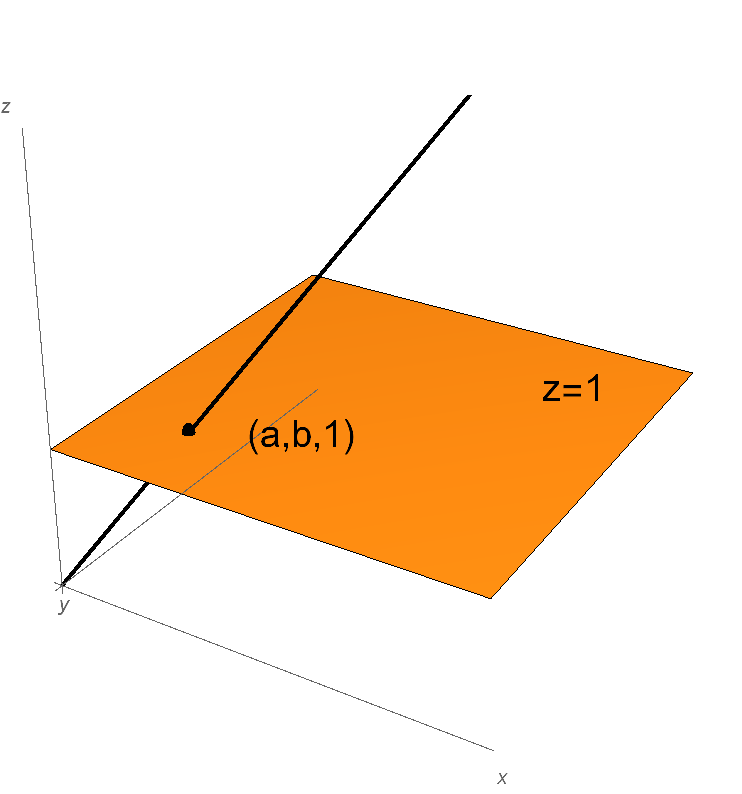
\includegraphics[width=0.6\textwidth]{images/projektivna_ravnina_mathematicafix.pdf}
% \caption[caption za v kazalo]{Dolg caption pod sliko}
  \caption[Primer točke v projektivni ravnini.]{Točka [a,b,1] v projektivni ravnini.}
  \label{fig:ravnina}
\end{figure}


\begin{definicija}
Polinom $P$ je \emph{homogen} stopnje $d$, če velja $$P(\lambda x,\lambda y, \lambda z) = \lambda ^d P(x,y,z) \text{ za vse } \lambda \in \F.$$.
\end{definicija}

\begin{definicija}
\emph{Algebraična krivulja}, podana s homogenim polinomom $P$, je množica točk 
$$\mathcal{C}_P= \{ A \in \mathbb{P}^2, P(A) = 0 \}.$$
\end{definicija}

\emph{Kubična krivulja} je algebraična krivulja, podana s homogenim polinomom stopnje 3. V splošnem je polinom oblike
\begin{align}
&{} a_{300}x^3+a_{210}x^2y+a_{201}x^2z+a_{120}xy^2+a_{102}xz^2+ \nonumber \\
&{}+a_{012}yz^2+a_{030}y^3+a_{003}z^3+a_{111}xyz+a_{021}y^2z, \nonumber
\end{align}
kjer so $a_{ijk} \in \F$.
Ta zapis vsebuje $10$ koeficientov, vendar se lahko v gladkih primerih polinom poenostavi z ustrezno zamenjavo spremenljivk.
\begin{definicija}
Algebraična krivulja je \emph{gladka}, če nima singularne točke.
\end{definicija}

\begin{izrek}[\protect{\cite{Gibson1999}, Izrek 15.2}]
Enačbo gladke kubične krivulje nad algebraično zaprtim poljem lahko zapišemo v Weierstrassovi obliki
$$y^2z = x^3 + axz^2 + bz^3.$$
\end{izrek}

\begin{trditev}[\protect{\cite{Silverman2009}, Trditev 1.4}]
Kubična krivulja v Weierstrassovi obliki je gladka natanko tedaj, ko velja
$$\Delta = -16(4a^3+27b^2) \neq 0.$$
\end{trditev}

\begin{opomba}
Gladki kubični krivulji  velikokrat rečemo tudi \emph{eliptična krivulja}.
\end{opomba}

\begin{primer}
Polinom $P(x,y,z) = z^2y-x^3$ je homogen polinom stopnje $3$. Rešitve enačbe $z^2y-x^3 = 0$ pa podajajo točke na kubični krivulji.
\begin{figure}[t]
  \centering
\begin{minipage}{.45\textwidth}
\centering
  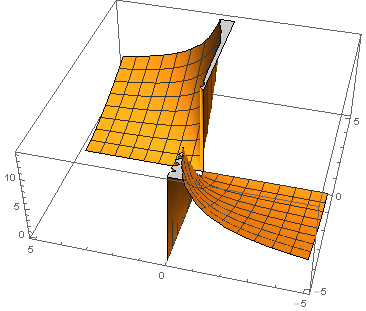
\includegraphics[width=0.8\textwidth]{images/krivulja.png}
  \caption[Primer algebraične krivulje.]{Algebraična krivulja $\mathcal{C}$ podana s polinomom $z^2y-x^3$.}
  \label{fig:krivulja}
\end{minipage}%
\hfill
\begin{minipage}{.45\textwidth}
\centering
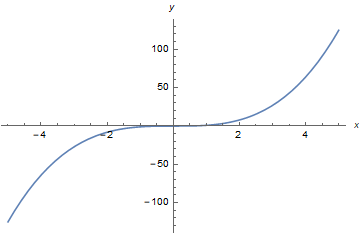
\includegraphics[scale=0.5]{images/projektivnaz.png}
\caption[Presek algebraične krivulje z ravnino $z=1$.]{Presek $\mathcal{C}$ z ravnino $z=1$.}
\label{fig:projektivnaz}
\end{minipage}
\end{figure}


\begin{figure}[t]
\centering
\begin{minipage}{.45\textwidth}
\centering
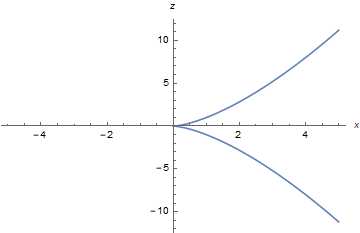
\includegraphics[scale=0.5]{images/projektivnay.png}
\caption[Presek algebraične krivulje z ravnino $y=1$.]{Presek $\mathcal{C}$ z ravnino $y=1$.}
\label{fig:projektivnay}
\end{minipage}%
\hfill
\begin{minipage}{.45\textwidth}
\centering
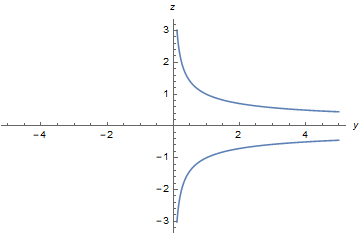
\includegraphics[scale=0.5]{images/projektivnax.png}
\caption[Presek algebraične krivulje z ravnino $x=1$.]{Presek $\mathcal{C}$ z ravnino $x=1$.}
\label{fig:projektivnax}
\end{minipage}
\end{figure}
Na zgornjih slikah lahko vidimo, kako krivuljo predstavimo v projektivni ravnini, ter njene preseke z različnimi afinimi ravninami.

\end{primer}



V nadaljevanju nas bodo zanimale predvsem kubične krivulje v končnem polju $\mathbb{Z}/p\mathbb{Z} \cong \Fq{p}$, za neko praštevilo $p$.

\begin{definicija}
Za dani števili $a$, $b \in \mathbb{Z}/p\mathbb{Z}$ je \emph{kubična krivulja} nad poljem $\mathbb{Z}/p\mathbb{Z}$ množica točk
$$E_{(a,b)}(\mathbb{Z}/p\mathbb{Z}) =\left\{ [x,y,z] \in \PP^2(\mathbb{Z}/p\mathbb{Z}): y^2z=x^3+axz^2+bz^3 \right\} .$$
Drugače povedano, afina kubična krivulja je množica rešitev Weierstrassove enačbe
$$y^2=x^3+ax+b,$$
pri čemer upoštevamo zvezo med afinimi in projektivnimi koordinatami točk:
$$(x,y)\in (\Z/p\Z)^2 \Leftrightarrow [x,y,1]\in \PP^2(\Z/p\Z).$$

\end{definicija}

\subsection{Tonelli-Shanks}
V algoritmih bomo velikokrat potrebovali naključno točko na krivulji. S pomočjo algoritma Tonelli-Shanks \cite{Tonelli1891} bomo točko na krivulji lahko učinkovito poiskali. Naj bo $p$ modul po katerem računamo.
Če privzamemo, da lahko naključno izberemo število $0 \leq x \leq p$, potem nas zanima, kako učinkovito izberemo naključno točko $(x,y)$ na krivulji podani z enačbo
$y^2 = x^3 +ax+b \ \text{mod } p$. Ideja je preprosta. Naključno generirajmo koordinato $x$ in nato poizkusimo rešiti enačbo $y^2 = X \ \text{mod } p$, če tak $y$ obstaja. V nasprotnem primeru generiramo novo $x$ koordinato in poizkusimo ponovno. Problem se torej skriva le v reševanju kvadratne enačbe. Tu pa nam pomaga Tonneli-Shankov algoritem, ki učinkovito reši zgornjo enačbo.

\begin{trditev}
Naj bo $p > 2$ praštevilo. Če je $n \in \F_p$ kvadratični ostanek po modolu $p$, potem nam Tonelli-Shanks algoritem vrne $r \in \F_p$, tako da velja $n = r^2$.

\end{trditev}

\begin{algorithm}[H]
\caption[Tonelli]{Tonelli-Shanks}
\label{alg:Tonelli}

\begin{algorithmic}
\State Vhod: praštevilo $p$, $n \in \F_p$.
\State Izhod: $r \in \F_p$, za katerega velja $r^2=n$, če ta obstaja
\State Najdi tak $z \in F_p$, da $z$ ni kvadrat
\State Poišči $s,Q$, tako da $p-1 = Q2^s$
\State $M = s,c = z^Q,t = n^Q,R=n^{\frac{Q+1}{2}}$
\While {True}
	\If {$t=0$}
		\State \Return $r=0$
	\ElsIf {$t=1$}
		\State \Return $r=R$
	\Else
		\State Poišči $0<i<M$, da velja $t^{2^i} = 1$
		\State  $M = i,c = b^2,t = tb^2,R=Rb$
	\EndIf
\EndWhile
\end{algorithmic}
\end{algorithm}

\begin{opomba}
V algoritmu \ref{alg:Tonelli} lahko prvi korak izvedemo tako, da preiskušamo naključne $g\in \F_p$, dokler ne velja $g^{(p-1)/2} = -1$.
\end{opomba}

\begin{opomba}
Števili $s, Q$ iz algoritma poiščemo tako, da število $p-1$ razpolavljamo dokler ne dobimo števila, ki ni deljivo z dva. To število je $Q$. Število korakov, ki smo jih naredili pa je $s$.
\end{opomba}


Algoritem \ref{alg:Tonelli} v povprečju potrebuje
$$2N+2K+\frac{s(s-1)}{4}+\frac{1}{2^{s-1}}-9$$
množenj. Tu $N$ predstavlja število binarnih števk števila $p$, $K$ pa predstavlja število enic v binarnem zapisu \cite{Tornaria2002}.

\subsection{Struktura grupe na kubičnih krivuljah}


Za definicijo grupe na kubičnih krivuljah nad $\C$ najprej uvedimo pomožno operacijo

$$\ast : \mathcal{C}_P \times \mathcal{C}_P \rightarrow \mathcal{C}_P,$$
tako da za poljubni točki $A$, $B$ na krivulji velja:

\[ A \ast B =
\begin{cases}
A & \quad \text{če je } A=B \ \text{prevoj},\\
C & \quad \text{če je } \overline{AB} \cap \mathcal{C}_P = \left\{ A,B,C \right\},\\
A & \quad \text{če je } \overline{AB} \ \text{tangenta v } A,\ \text{ter} \ A \neq B,\\
B & \quad \text{če je } \overline{AB} \ \text{tangenta v } B,\ \text{ter} \ A \neq B,\\
C &\quad \text{če je } A=B \  \text{in}\ \{\text{tangenta v A}\} \cap \mathcal{C}_P = \left\{ A,C \right\}.\\
\end{cases}
\]
Intuitivno operacija $\ast$ vrne tretjo točko v preseku premice skozi $A$ in $B$ in $\mathcal{C}_P$, kar lahko vidimo na sliki \ref{fig:adicija}. Poglejmo si še nekaj lastnosti operacije $\ast$. Dokaze sledečih trditev najdemo v \cite[Poglavje 17.3]{Gibson1999}.

\begin{trditev}
\label{last zvezda}
Operacija $\ast$ ima naslednje lastnosti:

\begin{itemize}
\item komutativnost: $ A \ast B = B \ast A$,
\item absorpcija: $(A \ast B ) \ast A = B$,
\item $((A \ast B) \ast C ) \ast D = A \ast ((B \ast D)\ast C)$.
\end{itemize}
\end{trditev}

\begin{izrek}
Kubična krivulja ($\mathcal{C}_P$,$+$) je Abelova grupa za operacijo

\begin{table}[ht]
\centering
\begin{tabular}{llll}
$+:$ & $\mathcal{C}_P \times \mathcal{C}_P$ & $\rightarrow$ & $\mathcal{C}_P$ \\
& $(A,B)$ & $\mapsto$ & $(A\ast B)\ast O$ ,
\end{tabular}
\end{table}
kjer je $O$ poljubna izbrana točka na krivulji $ \mathcal{C}_P$.
\end{izrek}

\begin{proof}
S pomočjo trditve \ref{last zvezda} dokažimo, da je ($\mathcal{C}_P$,$+$) res Abelova grupa.

\begin{itemize}
\item Operacija $+$ je komutativna:
$$A+B = (A \ast B ) \ast O = (B \ast A) \ast O = B+A.$$
\item Točka O je nevtralni element:
$$A+O=(A \ast O) \ast O = A.$$
\item Nasprotni element A definiramo kot $-A = A \ast (O \ast O )$ in preverimo:
\begin{align}
A + (-A) &{} = (A \ast (A \ast (O \ast O))) \ast O \nonumber \\
&{} = (O \ast O) \ast O \nonumber \\
&{} = O, \nonumber
\end{align}
kjer smo uporabili absorbcijo.
\item Asociativnost $(A + B) + C = A + (B + C)$ dokažemo z računom:
\begin{align}
(A + B) + C &{} = ((A + B) \ast C) \ast O \nonumber \\
&{} = (((A \ast B) \ast O) \ast C) \ast O \nonumber \\
&{} = (A \ast ((B \ast C) \ast O)) \ast O \nonumber \\
&{} = (A \ast (B + C)) \ast O = A + (B + C). \nonumber \qedhere
\end{align}
\end{itemize}
\end{proof}

Ta definicija operacije nudi eleganten geometrijski opis strukture grupe, za numerično računanje pa ni primerna. Možno pa je izpeljati formule, s katerimi eksplicitno
izračunamo vsoto dveh točk, v kolikor imamo kubično krivuljo v Weierstrassvi obliki.

\begin{lema}[Seštevanje točk na Weierstrassovi kubični krivulji]
\label{sestevanje}
Naj bo $\mathcal{C}_P$ afina krivulja v Weierstrassovi obliki $y^2 = x^3 + \alpha x^2 + \beta x + \gamma$, ter $O$ prevoj v neskončnosti. Če sta $A_1 = (a_1,b_1)$ in $A_2 = (a_2,b_2)$ točki na afinem delu $\mathcal{C}_P$, potem za $A_3 = A_1 + A_2 = (a_3,b_3)$ velja

%staro seštevanje
\begin{align}
&{} a_3 = \lambda ^2 - \alpha - a_1 - a_2, \nonumber \\
&{} b_3 = -\lambda a_3 - \mu, \nonumber
\end{align}
kjer sta 

$$
\lambda =
\begin{cases}
\frac{b_1 - b_2}{a_1 - a_2} & \quad \text{če } a_1 \neq a_2 ,\\
\frac{3a_1^2+ 2 \alpha a_1 + \beta}{2b_1} & \quad \text{sicer}\\
\end{cases}
\quad
\text{ in }
\quad
\mu = b_1 - \lambda a_1.
$$

%\begin{itemize}
%\item Če $a_1 \neq a_2$, potem
%$$a_3 = m^2-a_1-a_2, \ b_3 = m(a_1-a_3)-b_1, \text{ kjer velja } m= \frac{b_2-b_1}{a_2-a_1}.$$
%\item Če $a_1=a_2$, ampak $b_1 \neq b_2$, potem $A_1+A_2 = O$.
%\item Če $A_1 = A_2$ in $b_1 \neq 0$, potem
%$$a_3 = m^2-2a_1, \ b_3 = m(a_1-a_3)-b_1, \text{ kjer velja } m= \frac{3a_1^2+\alpha}{2b_1}.$$
%\item Če je $A_1 = A_2$ in $b_1 = 0$, potem $A_1 + A_2 = O$.
%\end{itemize}
%
%Poleg tega pa definiramo še 
%$$A_1+O = A_1,$$
%za vse točke $A_1$ na $E$.

\end{lema}


\begin{opomba}
Če krivuljo $\mathcal{C}_P$ predstavimo v projektivni ravnini, torej kot ničle homogenega polinomoma $y^2z=x^3+\alpha x^2z+\beta xz^2+ \gamma z^3$, je prevoj $O=[0,1,0].$
Opazimo, da točke $O = [0,1,0]$ ni možno predstaviti v afini ravnini $z=1$, zato bomo v nadaljevanju pisali $O = \infty$.
\end{opomba}

\begin{primer}
Na sliki \ref{fig:adicija} je v afini ravnini $z=1$ prikazano kako grafično seštevamo točke na Weierstrassovi kubiki $y^2z-x(x-z)(x+z)=0$. Sešteti želimo točki $A =[-1,0,1]$ in $B=[2,\sqrt{6},1] $.
\\


\begin{figure}[h]
  \centering
  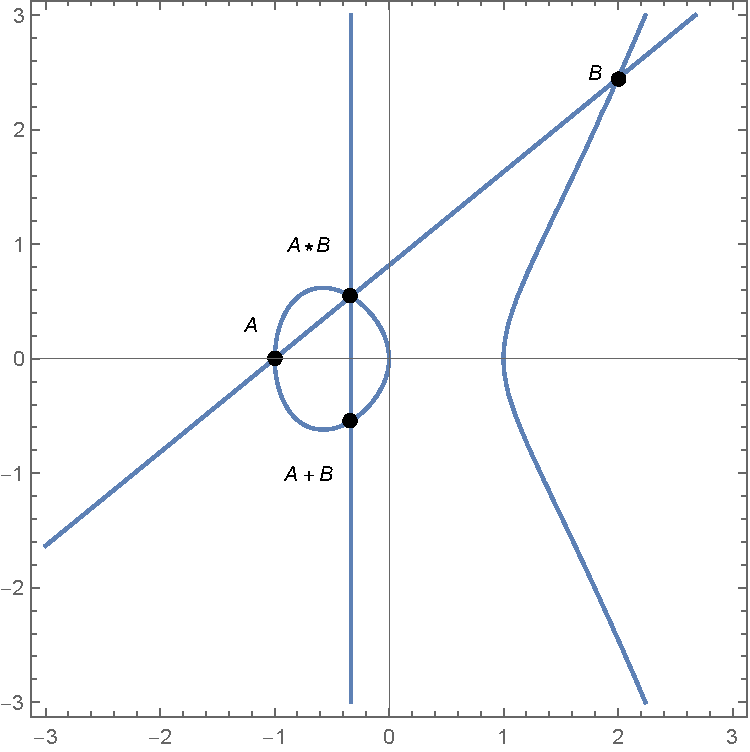
\includegraphics[width=0.8\textwidth]{images/sestevanje_tock_mathematicafix.pdf}
  \caption[Grafično seštevanje.]{Grafično seštevanje točk na kubični krivulji.}
  \label{fig:adicija}
\end{figure}

\end{primer}



\begin{primer}
Seštejmo točki $A =(-1,0),B=(2,\sqrt{6}) $ na Weierstrassovi kubični krivulji $y^2z-x(x-z)(x+z)=0$ v preseku z afino ravnino $z=1$ še računsko z uporabo zgornje leme \ref{sestevanje}.

Dobimo $y^2 = x^3-x,$
torej je $\alpha = 0$, $\beta = -1$ in $\gamma=0$. Izračunajmo sedaj $\lambda$ in $\mu$, pri čemer upoštevamo prvi predpis, saj sta x-koordinati točk različni:
$$\lambda = \frac{-\sqrt{6}}{-1-2} = \frac{\sqrt{6}}{3},$$

$$\mu = 0 - \frac{\sqrt{6}}{3} (-1) = \frac{\sqrt{6}}{3}.$$

Koordinati vsote $A+B=(x,y)$ sta torej enaki

$$x = \frac{6}{9} - 0+1-2=-\frac{1}{3}$$

in

$$y = -\frac{\sqrt{6}}{3}(-\frac{1}{3})-\frac{\sqrt{6}}{3}=-\frac{2\sqrt{6}}{9} \doteq -0.5443.$$

Iskana točka $A+B \in \PP^2$ je torej enaka $[-\frac{1}{3},-\frac{2\sqrt{6}}{9},1]$. Dobljeni rezultat se ujema s točko, ki smo jo dobili z grafičnim seštevanjem.

\end{primer}


Poglejmo si še primer kubične krivulje nad poljem $\F_p$.

\begin{primer}
Naj bo $E$ krivulja oblike $y^2 = x^3+x-1$ nad poljem $\Z_5$. Poglejmo si kako izgledajo točke na krivulji $E$.

\begin{table}[H]
\centering
\begin{tabular}{c|c|c|c}
$x$      & $x^3+x-1$ & $y$      & Točke         \\ \hline
$0$      & $-1$      & $\pm 3$  & $(0,3),(0,2)$ \\
$1$      & $1$       & $\pm 1$  & $(1,1),(1,4)$ \\
$2$      & $4$       & $\pm 3$  & $(2,3),(2,2)$ \\
$3$      & $4$       & $\pm 3$  & $(3,3),(3,2)$ \\
$4$      & $2$       & /        & /            
\end{tabular}
\end{table}

\begin{figure}[ht]
  \centering
\begin{minipage}{.45\textwidth}
\centering
  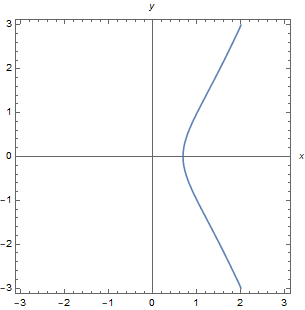
\includegraphics[scale = 0.5]{images/krivuljamod0.png}
  \caption[Primer algebraične krivulje.]{Algebraična krivulja $y^2 = x^3+x-1$ v $\R$.}
  \label{fig:krivuljamod0}
\end{minipage}%
\hfill
\begin{minipage}{.45\textwidth}
\centering
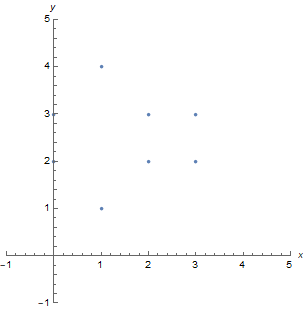
\includegraphics[scale=0.5]{images/krivuljamod1.png}
\caption[Presek algebraične krivulje z ravnino $z=1$.]{Algebraična krivulja $y^2 = x^3+x-1$ v $\Z_5$.}
\label{fig:krivuljamod1}
\end{minipage}
\end{figure}

Izračunajmo sedaj še $(2,3)+(1,1)$. Uporabimo formule v lemi \ref{sestevanje}, tako dobimo
\begin{align}
\lambda &{}=\frac{3-1}{2-1} = \frac{2}{1} = 2, \nonumber \\ 
%m &{}= \frac{1-3}{1-2} = \frac{3}{4} = 3\cdot 4 = 2, \nonumber \\
x_3 &{} = 4-2-1 = 1, \nonumber \\
\mu &{}= 3-2\cdot 2 = -1 = 4, \nonumber \\
y_3 &{} = -2(1)-4 = 4. \nonumber
\end{align}

$(2,3)+(1,1)$ je torej enako $(1,4)$ na krivulji $E$.

\end{primer}



\newpage

%%%%%%%%%%%%%%%%%%%%%%%%%%%%%%%%%%%%%%%%%%%%%%%%%%%%%%%%%%%%%%%%%%%%%%%%%%%%%%%%%%%%%%
%DELITELJI
%%%%%%%%%%%%%%%%%%%%%%%%%%%%%%%%%%%%%%%%%%%%%%%%%%%%%%%%%%%%%%%%%%%%%%%%%%%%%%%%%%%%%%

\section{Delitelji}

Pri konstrukciji Weilovega parjenja bodo pomembno vlogo igrali tako imenovani delitelji. V tem poglavju bomo navedli nekaj definicij in lastnosti, ki jih bomo potrebovali v kasnejših poglavjih. Uporabljali bomo terminologijo, ki jo lahko najdemo v \cite{Washington2008}.

\begin{definicija}
Naj bo $K$ polje in naj bo $P$ točka na krivulji $\E{\overline{K}}$. Za vsako točko $P$ definirajmo formalen simbol $[P]$. \emph{Delitelj} $D$ na krivulji $E$ je končna linearna kombinacija takih simbolov s celoštevilskimi koeficienti
$$D = \sum_{j}a_j[P_j], \ a_j \in \Z.$$

\end{definicija}

Iz same definicije sledi, da je delitelj element Abelove grupe generirane s simboli $[P]$. Označimo to grupo z $\DIV{E}$.


\begin{definicija}
Definirajmo \emph{vsoto} in \emph{stopnjo} delitelja kot
$$\SUM{\sum_{j}a_j[P_j]} = \sum_ja_jP_j \ \in \E{\overline{K}},$$
$$\DEG{\sum_{j}a_j[P_j]} = \sum_ja_j \ \in \Z.$$

\end{definicija}


\begin{definicija}
Naj bo $E$ eliptična krivulja nad poljem $K$. \emph{Funkcija} na $E$ je racionalna funkcija $$f(x,y) \in \ \overline{K},$$ ki je definirana za vsaj eno točko na $\E{\overline{K}}$. Funkcija torej zavzame vrednosti v $\overline{K}$.
\end{definicija}

\begin{opomba}
Naj bo $E$ podana z enačbo $y^2 = x^3+ax+b$. Racionalna funkcija $\frac{1}{y^2-x^3-ax-b}$ torej ne predstavlja funkcije na $E$, saj ni definirana za nobeno točko na $E$.

\end{opomba}

\begin{trditev}[\protect{\cite{Silverman2009}, Trditev 4.3}]
\label{trd:red}
Naj bo $P$ točka na krivulji $E$. Potem obstaja funkcija $u_P$, kateri rečemo uniformizator, z lastnostjo $u_P(P) = 0$, za katero velja, da lahko vsako funkcijo $f(x,y)$ nad $E$ zapišemo kot
$$f = u^r_Pg, \text{ za nek } r\in \Z, \text{ kjer } g(P) \neq 0 \text{ in } \frac{1}{g(P)} \neq 0.$$
\end{trditev}

\begin{definicija}
Številu $r$ iz trditve \ref{trd:red} rečemo \emph{red} funkcije $f$ v točki $P$ in ga označimo z $\ORDp{f}{P}$.
\end{definicija}

\begin{primer}
Naj bo $y^2 = x^3-x$ eliptična krivulja in naj bo $f(x,y) = x$. Za točko $P = (0,0)$ izberimo $u(x,y) = y$. Očitno je $u(0,0) = 0$. Nad eliptično krivuljo velja 
$$y^2 = x^3-x = x(x^2-1),$$ 
od tod sledi $x = y^2\frac{1}{x^2-1}$ nad E.
Prav tako velja, da $1/(x^2-1) \neq 0$ v točki $(0,0)$. Od tod sledi, da je red funkcij $x$ in $x/y$ enak
$$\ORDp{x}{(0,0)} = 2\text{ in }  \ORDp{x/y}{(0,0)}= 1.$$

Red funkcije je lahko tudi nepozitiven. Vzemimo funkcijo $1/x$. Enačbo krivulje prepišimo v obliko $\frac{1}{x} = \frac{1}{y^2}(x^2-1)$. To pomeni, da je red v točki $P=(0,0)$ enak
$$\ORDp{1/x}{(0,0)} = -2.$$

Poglejmo si še red funkcije $x/y^2$. Enačbo krivulje prepišimo v obliko $\frac{x}{y^2} = \frac{1}{x^2-1}$. Tu lahko vzamemo za uniformizator poljubno funkcijo, ki zadošča pogoju $u(P) = 0$, saj nastopa s potenco $0$. Torej je red funkcije $x/y^2$ v točki $P=(0,0)$ enak
$$\ORDp{x/y^2}{(0,0)} = 0.$$
\end{primer}

\begin{definicija}
Točki $P$ rečemo \emph{ničla} funkcije $f$, če je $\ORDp{f}{P} > 0$ in \emph{pol}, če je $\ORDp{f}{P} < 0$
\end{definicija}

\begin{definicija}
Naj bo $f$ funkcija nad $E$, ki ni identično enaka $0$. Definirajmo \emph{delitelj} funkcije $f$ kot
$$\Div{f} = \sum_{P\in \E{\overline{K}}} \ORDp{f}{P}[P] \in \DIV{E}.$$
\end{definicija}


\begin{trditev}[\protect{\cite{Washington2008}, Trditev 11.1}]
\label{trditev 11.1}
Naj bo $E$ eliptična krivulja in naj bo $f$ funkcija na $E$, ki ni identično enaka $0$. Potem veljajo naslednje trditve:
\begin{itemize}

\item $f$ ima le končno mnogo ničel in polov,
\item $\DEG{\Div{f}}=0$,
\item če $f$ nima ničel ali polov, potem je $f$ konstantna.
\end{itemize}


\end{trditev}

\begin{izrek}
\label{izrek 11.2}
Naj bo $E$ eliptična krivulja. Naj bo $D$ delitelj nad $E$ z $\DEG{D} = 0$. Potem obstaja taka funkcija $f$ na $E$ z lastnostjo
$$\Div{f} = D$$
natanko tedaj, ko
$$\SUM{D} = \text{točka }\infty.$$

\end{izrek}

\begin{proof}
Pokažimo najprej, da je možno $[P_1]+ [P_2]$ zapisati kot $$[P_1+P_2] + [\infty] + \text{delitelj neke funkcije}.$$
Recimo, da imamo tri kolinearne točke $P_1,P_2,P_3$ na krivulji $E$, ki ležijo na premici $ax+by+c = 0$.
Naj bo $f(x,y) = ax+by+c$, potem ima funkcija $f$ ničle v točkah $P_1,P_2,P_3$. Če $b$ ni enak $0$, potem ima funkcija po trditvi \ref{trditev 11.1} trojni pol v $\infty$.
Velja torej $$\Div{ax+by+c} = [P_1]+[P_2]+[P_3]-3[\infty].$$
Ker se nahajamo na krivulji zapisani v Weierstrassovi obliki, kjer točko $-P$ dobimo z zamenjavo predznaka y-koordinate, ima premica skozi točki $P_3 = (x_3,y_3)$ ter $-P_3=(x_3,-y_3)$ enačbo $x-x_3=0$.
Po  trditvi \ref{trditev 11.1} ponovno velja
$$\Div{x-x_3} = [P_3]+[-P_3]-2[\infty].$$
Od tod sledi
$$\text{div}\left( \frac{ax+by+c}{x-x_3}\right) = \Div{ax+by+c} - \Div{x-x_3} =[P_1]+[P_2]-[-P_3]-[\infty].$$
Ker na krivulji velja $P_1+P_2 = -P_3$ (to sledi iz definicije seštevanja točk na krivulji), lahko zgornjo enačbo prepišemo v 
$$[P_1]+[P_2] = [P_1+P_2]+[\infty]+\Div{g}, \text{ kjer je } g=\frac{ax+by+c}{x-x_3}.$$ 


Hitro opazimo, da velja
$$\SUM{\Div{g}}= P_1+P_2-(P_1+P_2)-\infty = \infty.$$
Prav tako pa se iz zgornje enačbe vidi, da je $[P_1]+[P_2] = 2[\infty] + \Div{g}$, če velja $P_1+P_2 = \infty$. Zaradi tega je vsota vseh členov s pozitivnimi koeficienti v $D$ enaka vsoti nekega simbola $[P]$, večkratnika $[\infty]$, ter delitelja neke funkcije. Enako velja tudi za člene z negativnimi koeficienti. Od tod sledi
$$D = [P]-[Q]+n[\infty]+\Div{h},$$
kjer je $h$ kvocient produkta funkcij z lastnostjo $\SUM{\Div{g_i}} = \infty$. Zato velja tudi
\newline $\SUM{\Div{h}}= \infty$. Po trditvi \ref{trditev 11.1} velja $\DEG{\Div{h}}=0$, saj funkcija ni konstantna. Imamo torej $$0 = \DEG{D} = 1-1+n+0=n.$$
Od tod sledi
$$D = [P]-[Q] + \Div{h}.$$
Prav tako velja
$$\SUM{D} = P-Q+\SUM{\Div{h}} = P-Q,$$
ker je $\infty$ nevtralni element Abelove grupe na $E$.
Predpostavimo sedaj, da velja $\SUM{D} = \infty$. Potem je $P-Q = \infty$, zato mora veljati $P=Q$ in $D = \Div{h}$. Za dokaz v obratno smer predpostavimo, da je $D = \Div{f}$ za neko funkcijo f. Potem je
$$[P]-[Q] = \Div{f/h}.$$
Od tod po spodnji lemi \ref{lema 11.3} sledi, da je $P = Q$ in torej $\SUM{D} = \infty$.

\end{proof}

\begin{lema}[\protect{\cite{Washington2008}, Lema 11.3}]
\label{lema 11.3}
Naj bosta $P,Q \in \E{\overline{K}}$, ter $h$ funkcija na $E$ za katero velja
$$\Div{h}=[P]-[Q].$$
Potem sledi $P=Q$.
\end{lema}
\newpage

\section{Krivulje končnega reda}
%%%%%%%%%%%%%%%%%%%%%%%%%%%%%%%%%%%%%%%%%%%%%%%%%%%%%%%%%%%%%%%%%%%%%%%%%%%%%%%%%%%%%%
%Torzijske točke
%%%%%%%%%%%%%%%%%%%%%%%%%%%%%%%%%%%%%%%%%%%%%%%%%%%%%%%%%%%%%%%%%%%%%%%%%%%%%%%%%%%%%%
\subsection{Torzijske točke}

\begin{definicija}
Naj bo $E$ eliptična krivulja nad poljem $K$, ter naj bo $n\in \N$. \emph{Torizjske točke} reda $n$, so točke v množici
$$E[n] = \{ P \in \E{\overline{K}} | nP = \infty \}.$$
\end{definicija}

Struktura torzijskih točk je opisana v naslednjem izreku.

\begin{izrek}
\label{IzrekTor}
Naj bo $E$ eliptična krivulja nad poljem $K$ in naj bo $n \in \N$. Če karakteristika polja $K$ ne deli $n$ oziroma je enaka $0$, potem je
$$E[n] \cong \mathbb{Z}_n \oplus \mathbb{Z}_n.$$

Zapišimo $n=p^rn'$, kjer $p$ ne deli $n'$. Če je karakteristika $K$ enaka $p >0$ in $p|n$, potem velja
$$E[n] \cong \mathbb{Z}_{n'} \oplus \mathbb{Z}_{n'} \text{ ali } E[n] \cong \mathbb{Z}_n \oplus \mathbb{Z}_{n'}.$$

\end{izrek}

Izrek \ref{IzrekTor} bomo dokazali v zadnjem razdelku tega poglavja.

\subsection{Endomorfizmi}
\label{endomorfizmi}

\begin{definicija}
Naj bo $K$ polje nad katerim je definirana eliptična krivulja $E$.
\emph{Endomorfizem} na $E$ je homomorfizem $\alpha: \E{\overline{K}} \rightarrow \E{\overline{K}} $, ki je podan z racionalno funkcijo. Torej obstajata racionalni funkciji $R_1$ in $R_2$ s koeficienti v $\overline{K}$ za kateri velja
$$\alpha(x,y) = (R_1(x,y),R_2(x,y)),$$
za vse $(x,y) \in \E{\overline{K}}$.
\end{definicija}

\begin{primer}
Naj bo $E$ krivulja podana z $y^2 = x^3+ax+b$, ter naj bo $\alpha(P) = 2P$. Tako definiran $\alpha$ je očitno homomorfizem. Po lemi \ref{sestevanje} pa obstajajo racionalne funkcije za seštevanje točk na kubičnih krivuljah, zato je $\alpha$ tudi endomorfizem.
\end{primer}

Zaradi različnih možnih oblik racionalnih funkcij bo priročno, če bomo zapis endomorfizmov standardizirali, ter bomo od tod naprej privzeli, da so vsi endomorfizmi zapisani v enotni obliki.
V racionalni funkciji $R(x,y)$ lahko, zato ker se nahajamo na Weierstrassovi krivulji, vse sode potence $y$ zamenjamo z $x^3+ax+b$ na primerno potenco. Zaradi tega lahko $R(x,y)$ zapišemo kot
$$R(x,y) = \frac{p_1(x)+p_2(x)y}{p_3(x)+p_4(x)y}.$$
Če sedaj še pomnožimo števec in imenovalec s $p_3-p_4y$ ter potem zamenjamo $y^2$ z $x^3+ax+b$, dobimo izraz oblike
$$R(x,y) = \frac{q_1(x)+q_2(x)y}{q_3(x)}.$$
Za točke na Weierstrassovi krivulji velja $-(x,y) = (x,-y)$, kjer $-(x,y)$ označuje nasprotni element točke $(x,y)$. Od tod sklepamo, da za vsak endomorfizem $\alpha = (R_1,R_2) $ nad $E$ velja
$$R_1(x,-y) = R_1(x,y), \ R_2(x,-y) = -R_2(x,y).$$
To sledi iz dejstva, da je $\alpha$ homomorfizem in velja
$$\alpha(x,-y) = \alpha(-(x,y)) = -\alpha(x,y).$$
To pa pomeni, da se da $\alpha(x,y)$ zapisati kot
$\alpha(x,y) = (r_1(x),r_2(x)y),$
kjer sta $r_1,r_2$ racionalni funkciji.

Če sedaj zapišemo $r_1(x)$ kot
$$r_1(x) = \frac{p(x)}{q(x)},$$
potem lahko definiramo še nekaj pojmov. 

\begin{definicija}
\emph{Stopnja} endomorfizma je  definirana kot
$$
\DEG{\alpha} =
\begin{cases}
\max \{ \deg{p(x)},\deg{q(x)} \} & \text{če }\alpha \not\equiv 0, \\
0 & \text{če } \alpha \equiv 0.
\end{cases}
$$
\end{definicija}

\begin{definicija}
Netrivialni endomorfizem $\alpha$ je \emph{separabilen}, če je odvod $r'_1(x) \not \equiv 0$.
\end{definicija}

Poglejmo si na primeru, kako določimo stopnjo, ter ali je enodmorfizem seperabilen.

\begin{primer}
Če vzamemo endomorfizem iz prejšnjega primera $\alpha(P) = 2P,$ dobimo funkcijo
$$R_1(x,y) = \left(\frac{3x^2+a}{2y}\right)^2-2x.$$
To lahko preoblikujemo kot
\begin{align}
\left(\frac{3x^2+a}{2y}\right)^2-2x &{}= \frac{9x^4+6ax^2+a^2}{4y^2}-2x \nonumber \\
&{} = \frac{9x^4+6ax^2+a^2 - 2x(4(x^2+ax+b))}{4(x^2+ax+b)} \nonumber \\
&{} = \frac{x^4-2ax^2-8bx+a^2}{4(x^2+ax+b)}. \nonumber
\end{align}
Iz
$$r_1(x) = \frac{x^4-2ax^2-8bx+a^2}{4(x^2+ax+b)}$$
razberemo, da je stopnja $\DEG{\alpha} = 4$.

Poglejmo si še odvod $r'_1(x)$.
\begin{align}
r'_1(x) &{}=\frac{(4x^3-4ax-8b)4(x^3+ax+b)-(x^4-2ax^2-8bx+a^2)(12x^2+4a)}{16(x^2+ax+b)^2} \nonumber \\
&{} = \frac{-a^3 - 8 b^2 + 2 x^5 - 2 a^2 x (1 + x) + 4 b x^2 (2 + x) +  a (-4 b x + 3 x^4)}{4 (b + x (a + x))^2}. \nonumber
\end{align}
Števec zgornje enačbe pa ni identično enak $0$, torej je endomorfizem seperabilen.
\begin{opomba}
Če bi zgornje računali v $\F_2$, bi dobili primer endomorfizma, ki ni seperabilen.
\end{opomba}
\end{primer}

V nadaljevanju bomo potrebovali naslednji izrek, za katerega ne bomo podali dokaza.

\begin{izrek}[\protect{\cite{Washington2008}, Izrek 2.21}]
\label{izrek:2.21}
Naj bo $\alpha \neq 0$ seperabilni endomorfizem nad eliptično krivuljo $E$. Potem velja
$$\DEG{\alpha}= \# \text{Ker}(\alpha), \ \text{kjer \# označuje število točk, ki so v jedru } \alpha.$$
Če $\alpha \neq 0$ ni seperabilen, pa velja
$$\DEG{\alpha} > \# \text{Ker}(\alpha).$$
\end{izrek}

\subsection{Frobeniusov endomorfizem}

Naj bo $\F_q$ končno polje z algebraičnim zaprtjem $\overline{\F_q}$ in naj bo
\begin{align}
\phi_q:\overline{\F_q} &{} \rightarrow \overline{\F_q}, \nonumber \\
x &{} \mapsto x^q \nonumber
\end{align}
Frobeniusova preslikava na $\F_q$.
Če je eliptična krivulja $E$ definirana nad $\F_q$, potem $\phi_q$ deluje na točkah $E$ kot:
$$\phi_q(x,y) = (x^q,y^q) \text{ in } \phi_q(\infty) = \infty.$$

\begin{lema}
\label{lema:4.5}

Naj bo $E$ eliptična krivulja definirana nad $\F_q$. Za točke $(x,y) \in \E{\overline{\F_q}}$ velja
\begin{itemize}

\item $\phi_q(x,y) \in \E{\overline{\F_q}}$,
\item $(x,y) \in \E{\F_q}$ natanko tedaj ko je $\phi_q(x,y) = (x,y)$.


\end{itemize}

\end{lema}

\begin{proof}
Za dokaz leme bomo potrebovali lastnost $$(a+b)^q = a^q+b^q,$$ kjer je $q$ potenca karakteristike polja v katerem delamo. To sledi iz razvoja v vrsto in dejstva, da pri binomskih koeficientih velja
${q\choose i} \equiv 0$, za $1 \leq i \leq q-1$. To je res, ker pri zapisu binomskega koeficienta po krajšanju vedno ostane vsaj en $q$, ki je potenca karakteristike. 

Prav tako bomo potrebovali trditev \ref{algebra}, da za vse $a \in \F_q$ velja $a^q = a$. Dokaz tega sledi iz dejstva, da ima grupa vseh obrnljivih elementov $\F^{\times}_q$ red $q-1$, kar pomeni $a^{q-1} = 1$, za vse $a \in \F_q \neq 0$. To pa je ekvivalentno zgornji trditvi.

Lemo lahko brez težav dokažemo za krivulje v posplošeni Weierstrassovi obliki.
\begin{equation}
\label{enc:razWeier}
y^2+a_1xy+a_3y=x^3+a_2x^2+a_4x+a_6,
\end{equation}
kjer so $a_i \in \F_q$. Če to enačbo potenciramo na stopnjo $q$ in uporabimo zgornja dejstva, dobimo
$$(y^q)^2+a_1(x^qy^q)+a_3(y^q)=(x^q)^3+a_2(x^q)^2+a_4(x^q)+a_6.$$
To pa ravno pomeni, da točke oblike $(x^q,y^q)$ ležijo na krivulji podani z enačbo \ref{enc:razWeier}.

Za drugi del leme uporabimo dejstvo, da velja $x \in \F_q$ natanko tedaj, ko je $\phi_q(x) = x$. Smer iz leve v desno smo že dokazali zgoraj. Potrebujemo še dokaz v drugo smer. Ta pa sledi iz lastnosti, da ima polinom $X^q-X$ natanko $q$ različnih ničel v $\overline{\F_p}$. Ker pa množici
$$\{ \alpha \in \overline{\F_p} | \alpha^q = \alpha \} \text{ in } \F_q$$
vsebujeta $q$ elementov in je $\F_q$ vsebovana v drugi množici, sledi da sta enaki.

Od tod za točke $(x,y) \in \E{\Fq{q}}$ sledi
\begin{align}
(x,y) \in E(\F_q) &{}\Leftrightarrow x,y \in \F_q \nonumber \\
&{}  \Leftrightarrow \phi_q(x) = x \text{ in } \phi_q(y) = y  \nonumber \\
&{} \Leftrightarrow \phi_q(x,y) = (x,y). \nonumber
\end{align} 

\end{proof}

\begin{trditev}
\label{trd:3.16}
Naj bo $E$ eliptična krivulja definirana nad $\Fq{q}$.
Naj bosta $\alpha,\beta$ endomorfizma na $E$ ter $a,b \in \Z$. Definirajmo endomorfizem
$$(a\alpha+b\beta)(P) = a\alpha(P)+b\beta(P).$$
Potem velja
$$\DEG{a\alpha+b\beta} = a^2\DEG{\alpha}+b^2\DEG{\beta} + ab\text{(}\DEG{\alpha+\beta}-\DEG{\alpha}-\DEG{\beta}\text{)}.$$
\end{trditev}

\begin{opomba}
Naj $n \in \N$ ne deli karakteristike $K$. Ker velja $E[n] \cong \Z_n \bigoplus \Z_n$, lahko za $E[n]$ izberemo neko bazo $\{ \beta_1, \beta_2\}$. To pomeni, da lahko vsak element $E[n]$ zapišemo kot $m_1\beta_1 + m_2\beta_2$, za $m_1, m_2 \in \Z_n$. Homomorfizem $\alpha: \E{\overline{K}} \rightarrow \E{\overline{K}}$ preslika $E[n]$ v $E[n]$. Zato obstajajo števila $a,b,c,d \in \Z_n$, da velja
$$\alpha(\beta_1) = a\beta_1+b\beta_2, \ \alpha(\beta_2) = c\beta_1+d\beta_2.$$
To pa ravno pomeni, da se lahko vsak tak homomorfizem $\alpha$ predstavimo z matriko oblike
$$\alpha_n = \begin{bmatrix}
a & b \\
c & d
\end{bmatrix}.$$
\end{opomba}

\begin{proof}
Naj bo $n \in \Z$, število ki ni deljivo s karakteristiko polja. Predstavimo $\alpha,\beta$ z matrikami $\alpha_n,\beta_n$, glede na neko bazo $E[n]$.
Velja
\begin{align}
\text{det}(a\alpha_n+b\beta_n) &{}=  a^2\text{det}(\alpha_n)+b^2\text{det}(\beta_n) + ab(\text{det}(\alpha_n+\beta_n)-\text{det}(\alpha_n)-\text{det}(\beta_n)) \nonumber
\end{align}
za vse matrike $\alpha_n,\beta_n$.
Od tod sledi
\begin{align}
\DEG{a\alpha+b\beta} &{}\equiv a^2\DEG{\alpha}+b^2\DEG{\beta} + ab(\DEG{\alpha+\beta} \nonumber \\
&{}-\DEG{\alpha}-\DEG{\beta}) \MOD{n}. \nonumber
\end{align}
Ker to drži za neskončno mnogo $n$, v tej enačbi velja enakost.


\end{proof}

\begin{trditev}[\protect{\cite{Washington2008}, Trditev 4.7}]
\label{trd:4.7}
Naj bo $E$ definirana nad $\F_q$ in naj bo $n \geq 1$. Potem velja
\begin{itemize}
\item $\text{Ker}(\phi^n_q-1) = \E{\F_{q^n}}$.
\item Endomorfizem $\phi^n_q-1$ je seperabilen. Velja torej $\#\E{\F_{q^n}} = \DEG{\phi^n_q-1}$.
\end{itemize}
\end{trditev}

\begin{opomba}
$\phi^n_q$ predstavlja kompozicijo $\phi_q \circ \phi_q \circ \ldots \circ \phi_q$. Prav tako pa je $\phi^n_q-1$ endomorfizem, saj je množenje z $-1$ endomorfizem.
\end{opomba}

\begin{izrek}[Hasse \protect{\cite{Washington2008}, Izrek 4.2}]
\label{izr:Hasse}
Naj bo $E$ eliptična krivulja nad končnim poljem $\F_q$.  Potem red $\E{\F_q}$ zadošča zvezi
$$|q+1-\#\E{\F_q}| \leq 2\sqrt{q}.$$
\end{izrek}

\begin{opomba}
Hassejev izrek igra pomembno vlogo tudi pri iskanju velikosti grupe, saj nam poda zgornjo in spodnjo mejo. Velikost grupe pa potem nadaljno zožimo z dejstvom, da red elementa deli red grupe. 
\end{opomba}

\begin{lema}
\label{lema:hasse}
Naj bosta $r,s \in \Z$ tuji števili. Potem velja
$$\DEG{r\phi_q-s} = r^2q+s^2-rsa.$$
\end{lema}

\begin{proof}
Z uporabo trditve \ref{trd:3.16} dobimo
$$\DEG{r\phi_q-s} = r^2\DEG{\phi_q}+s^2\DEG{-1}+rs(\DEG{\phi_q-1}-\DEG{\phi_q}-\DEG{-1}).$$
Če sedaj uporabimo dejstvi $\DEG{\phi_q} = q,\ \DEG{-1} = 1$ ter $\DEG{\phi_q-1} = q+1-a$, željeni rezultat sledi.
\end{proof}

\begin{proof}[Dokaz izreka \ref{izr:Hasse}]
Po trditvi \ref{trd:4.7} lahko zapišemo
$$a=q+1-\#\E{\F_q} = q+1 -\DEG{\phi_q-1}.$$
Pokazati moramo $|a| \leq 2\sqrt{q}.$
Ker velja $\DEG{r\phi_q-s} \geq 0$, nam lema \ref{lema:hasse} implicira
$$q \left( \frac{r}{s} \right)^2-a\frac{r}{s}+1 \geq 0,$$
za vse $r,s$ za katere je $\text{gcd}(s,q)=1$. Množica racionalnih števil oblike $r/s$, ki zadoščajo tej lastnosti je gosta v $\R$. To lahko vidimo tako, da za $s$ vzamemo potenco števila $2$ ali $3$. Vsaj eno od teh števil bo tuje $q$, saj je $q$ moč končnega polja in je torej oblike $q = t^n$, za neko praštevilo $t$. Števila oblike $\frac{r}{2^m}$ ali $\frac{r}{3^m}$ pa so očitno gosta v $\R$. Zato velja
$$qx^2-ax + 1 \geq 0,$$
za vse $x\in \R$. To pa pomeni, da je diskriminanta polinoma negativna ali nič. Kar povedano z drugimi besedami pomeni
$$a^2-4q \leq 0.$$
To pa je ravno pogoj $|a|\leq 2\sqrt{q}$.


\end{proof}


\begin{izrek}[\protect{\cite{Washington2008}, Izrek 4.10}]
\label{izrek:4.10}
Naj bo E eliptična krivulja definirana nad $\F_q$. Naj bo $a = q+1-\#\E{\F_q} = q+1-\DEG{\phi_q-1}$. Potem velja
$$\phi^2_q-a\phi_q+q = 0,$$
gledano kot endomorfizem nad $E$. Prav tako pa je $a$ edino število $k$, za katerega velja
$$\phi^2_{q^n}-k\phi_{q^n}+q^n = 0.$$

Povedano drugače, velja naslednja lastnost. Naj bo $(x,y) \in  \overline{\F_q}$, potem velja
$$(x^{q^2},y^{q^2})-a(x^q,y^q)+q(x,y) = \infty,$$
obenem pa je $a$ edino število, tako da ta lastnost velja za vse $(x,y) \in \overline{\F_q} $. Velja še več
$$a \equiv Sled((\phi_q)_m) \text{ mod } m,$$
za vse $m$, ki zadoščajo $\text{gcd}(m,q)=1$.

\end{izrek}

\subsection{Red grupe nad eliptičnimi krivuljami}


Pogosto nas zanima, koliko točk leži na dani krivulji $E$. S pomočjo naslednje trditve bomo dobili preprost način kako izračunati $\# \E{\F_{q^n}}$, če poznamo $\# \E{\F_q}$.
Preostane še vprašanje kako izračunati $\# \E{\F_q}$. Enega od možnih načinov bomo opisali v opombi \ref{opo:MaliVeliki}, kot posledico algoritma Velik korak-majhen korak.




\begin{trditev}
\label{trd:4.12}
Naj bo $\# \E{\F_q} = q+1-a$, kot v izreku \ref{izrek:4.10}. Zapišimo $X^2-aX+q = (X-\alpha)(x-\beta)$. Potem velja
$$\# \E{\F_{q^{n}}} = q^n+1-(\alpha^n+\beta^n),$$
za vse $n \geq 1$.

\end{trditev}

Preden lahko dokažemo zgornjo trditev, bomo potrebovali še naslednjo lemo.

\begin{lema}
\label{lema:4.13}
Naj bo $s_n = \alpha^n +  \beta^n$. Potem velja $s_0 = 2,s_1 = a$ in $ s_{n+1} = as_n-qs_{n-1}$, za vse $n \geq 1$.

\end{lema}

\begin{proof}
Če je $n = 0$, potem lema očitno velja. Za $n=1$ lema sledi iz definicije $\alpha$ in $\beta$, ki sta ničli enačbe $X^2-aX+q$, ter uporabe Vietovih formul. Dokažimo lemo še za splošen $n$.
Ker sta $\alpha$ in $\beta$ ničli iste enačbe, lahko zapišemo $\alpha^2-a\alpha +q = 0$ in $\beta^2-a\beta+q=0$. Sedaj enačbi pomnožimo z $\alpha^{n-1}$ in $\beta^{n-1}$. S tem dobimo
$$\alpha^{n+1} = a\alpha^n +q\alpha^{n-1}\text{ in } \beta^{n+1} = a\beta^n +q\beta^{n-1}.$$
Če enačbi seštejemo, dobimo rekurzivno zvezo
$$s_{n+1} = as_n-qs_{n-1}.$$
\end{proof}

\begin{proof}[Dokaz trditve \ref{trd:4.12}]
Iz leme \ref{lema:4.13} takoj sledi, da velja $\alpha^n+\beta^n \in \N$. Naj bo $f$ funkcija

$$f(X) = (X^n-\alpha^n)(X^n-\beta^n) = X^{2n}-(\alpha^n+\beta^n)X^n+q^n.$$
Iz prve enakosti sledi, da funkcija $X^2-aX+q = (X-\alpha)(X-\beta)$ deli $f$. Po osnovnem izreku od deljenju lahko f zapišemo kot $f(X) = g(X)Q(x)+r(x)$, kjer je $g(X)= X^2-aX+q$. Prav tako pa ima kvocient $Q$ celoštevilske koeficiente. Po izreku \ref{izrek:4.10} velja

$$(\phi^n_q)^2 -(\alpha^n+\beta^n)\phi^n_q + q^n = f(\phi_q) = Q(\phi_q)(\phi^2_q-a\phi_q+q) = 0,$$
kjer je $\phi_q$ endomorfizem na $E$. Velja tudi $\phi^n_q = \phi_{q^n}$. Ponovno uporabimo izrek \ref{izrek:4.10}, od koder sledi, da obstaja natanko en $k \in \Z$, za katerega je
$\phi^2_{q^n}-k\phi_{q^n}+q^n=0$, in sicer, $k = q^n+1-\#\E{\F_{q^n}}$. Od tod torej sledi
$$\alpha^n+\beta^n = q^n+1-\#\E{\F_{q^n}}.$$

\end{proof}

\begin{primer}
Naj bo $E$ posplošena Weierstrassova krivulja podana s predpisom $y^2+xy = x^3+1$. S preprostim pregledom vseh možnosti vidimo, da je $\#\E{\F_2} = 4$. Izračunajmo sedaj $\#\E{\F_4}$. Po trditvi \ref{trd:4.12} moramo
$\#\E{\F_2}$ zapisati kot $q+1-a$. Sledi torej $a = 2+1-4 = -1$. Polinom je potem oblike
$$X^2+X+2 = \left( X-\frac{-1+\sqrt{-7}}{2}\right) \left(X-\frac{-1-\sqrt{-7}}{2}\right).$$
Za število točk na krivulji moramo poračunati še $s_2=\alpha^2+\beta^2$, pri čemer si lahko pomagamo z lemo \ref{lema:4.13}.
$$s_2 = as_1-qs_0 = (-1)^2-2\cdot2 = -3$$
Od tod sledi
$$\#\E{\F_{2^2}} = 2^2+1-s_2 = 4+1+3 = 8.$$
 Če naštejemo vse točke na $\E{\F_{4}} = \{ \infty,(0,1),(1,0),(1,1),(1,2),(3,0),(0,3),(1,3)\}$, vidimo da je naš rezultat pravilen.
Moč trditve \ref{trd:4.12} pa se skriva v velikih potencah. Če bi na primer želeli izračunati
$\E{\F_{2^{200}}}$ z naštevanjem točk ne bi prišli prav daleč. S pomočjo zgornje trditve in leme pa lahko hitro poračunamo
$$\left(\frac{-1+\sqrt{-7}}{2}\right)^{200}+ \left(\frac{-1-\sqrt{-7}}{2}\right)^{200} = -2534943693362688758337590430751,$$
od koder sledi
\begin{align}
\E{\F_{2^{200}}} &{}= 2^{200} + 1 +2534943693362688758337590430751 \nonumber \\
&{}= 1606938044258990275541962092343697546215565682541130425732128. \nonumber
\end{align}
\end{primer}
\subsection{Dokaz izreka \ref{IzrekTor}}
\begin{definicija}
Definirajmo $m$-ti \emph{deliteljski polinom} $\gamma_m \in \Z[x,y,a,b]$ kot


\begin{align}
\gamma_0 &{}= 0  \nonumber \\
\gamma_1 &{}= 1  \nonumber \\
\gamma_2 &{}= 2y  \nonumber \\
\gamma_3 &{}= 3x^4 + 6ax^2 + 12bx-a^2 \nonumber \\
\gamma_4 &{}= 4y(x^6+5ax^4+20bx^3-5a^2x^2-4abx-8b^2-a^3) \nonumber \\
\gamma_{2m+1} &{}= \gamma_{m+2}\gamma_{m}^3-\gamma_{m-1}\gamma_{m+1}^3 \text{ za } m \geq 2 \nonumber \\
\gamma_{2m} &{}= (2y)^{-1}\gamma_{m}(\gamma_{m+2}\gamma_{m-1}^2-\gamma_{m-2}\gamma_{m+1}^2)\text{ za } m \geq 3 \nonumber
\end{align}

\end{definicija}

\begin{lema}
Polinom $\gamma_{n}$ je element $\Z[x,y^2,a,b]$ za vse lihe $n$.  Za sode $n$ pa je $\gamma_{n}$ element \newline $2y\Z[x,y^2,a,b]$.

\end{lema}

\begin{proof}
Lemo dokažemo s pomočjo indukcije. Za $n \leq 4$ lema očitno velja. Obravnavajmo primera, ko je $n=2m$ in  $n=2m+1$ za nek $m\in\N$.
\begin{itemize}
\item{$n=2m$:}
Predpostavimo lahko, da je $2m>4$, saj vemo, da lema velja za $n\leq 4$, torej je $m>2$. Potem velja $2m>m+2$, kar pomeni, da vsi polinomi v definiciji $\gamma_{2m}$ zadoščajo indukcijski predpostavki. Če je $m$ sodo število, potem se $\gamma_{m},\gamma_{m+2},\gamma_{m-2}$ nahajajo v $2y\Z[x,y^2,a,b]$. Od tod pa sledi, da je tudi $\gamma_{2m} \in 2y\Z[x,y^2,a,b]$.
Če je $m$ lih, potem sta $\gamma_{m-1},\gamma_{m+1} \in 2y\Z[x,y^2,a,b]$. To pa pomeni, da je tudi  $\gamma_{2m} \in 2y\Z[x,y^2,a,b]$.
\item{$n=2m+1$:}
Primer obravnavamo podobno kot $n=2m$.


\end{itemize}


\end{proof}

Definirajmo še polinoma
\begin{align}
\phi_m &{}=x\gamma^2_m-\gamma_{m+1}\gamma_{m-1}, \nonumber \\
\omega_m &{} = (4y)^{-1}(\gamma_{m+2}\gamma^2_{m-1}-\gamma_{m-2}\gamma^2_{m+1}). \nonumber
\end{align}

Podobno kot pri polinomih $\gamma_m$, lahko tudi za $\phi_m$ in $\omega_m$ formuliramo lemo, katere dokaz bomo izpustili.

\begin{lema}
Polinom $\phi_{n}$ je element $\Z[x,y^2,a,b]$, za vse $n$. Če je $n$ lih, potem je $\omega_{n}$ element v \newline $y\Z[x,y^2,a,b]$. Za sode $n$ pa je $\omega_{n}$ element v $\Z[x,y^2,a,b]$.

\end{lema}

Predstavimo sedaj $\gamma_m, \omega_m, \phi_m$ kot polinome nad eliptičnimi krivuljami v Weierstrassovi obliki
$$E: y^2=x^3+ax+b.$$
Polinome v $\Z[x,y^2,a,b]$ lahko gledamo kot polinome v $\Z[x,a,b]$, tako da $y^2$ nadomestimo z $x^3+ax+b$.

\begin{opomba}
Polinoma $\gamma_n$ ni vedno možno predstaviti kot polinom spremenljivke $x$, saj je potenca $y$ odvisna od parnosti $n$. Vseeno pa velja, da lahko $\gamma^2_n$ vedno zapišemo kot polinom spremenljivke $x$.

\end{opomba}

\begin{izrek}[\protect{\cite{Washington2008}, Izrek 3.6}]

\label{izrek:3.6}
Naj bo $P = (x,y)$ točka na krivulji $y^2 = x^3+ax+b$, nad poljem s karakteristiko različno od $2$. Naj bo $n\in \N$, potem velja
$$nP = \left( \frac{\phi_n(x)}{\gamma^2_n(x)}, \frac{\omega_n(x,y)}{\gamma^3_n(x,y)}\right).$$


\end{izrek}

\begin{posledica}
\label{posledica:3.7}
Naj bo $E$ eliptična krivulja. Endomorfizem $E$ podan kot množenje z $n$, ima stopnjo $n^2$.
\end{posledica}

Brez dokazov formulirajmo še nekaj pomožnih trditev, ki jih bomo potrebovali za dokaz izreka \ref{IzrekTor}.

\begin{izrek}[\protect{\cite{Washington2008}, Izrek 2.22}]
\label{izrek:2.22}
Naj bo $E$ eliptična krivulja definirana nad poljem $K$. Naj bo $\alpha \neq 0$ endomorfizem na $E$. Potem je $\alpha: \E{\overline{K}} \rightarrow \E{\overline{K}}$ surjektivna preslikava.

\end{izrek}

\begin{trditev}[\protect{\cite{Washington2008}, Trditev 2.28}]
\label{trditev:2.28}
Naj bo $E$ eliptična krivulja definirana nad poljem $K$, ter naj bo $n\in \N$. Naj bo množenje z $n$ na $E$ podano z racionalnima funkcijama $R_n$ in $S_n$, kot v razdelku \ref{endomorfizmi},
$$n(x,y) = (R_n(x),yS_n(x))$$
za vse $(x,y) \in \E{\overline{K}}$. Potem velja
$$\frac{R'_n(x)}{S_n(x)} = n.$$
Od tod pa sledi, da je množenje z $n$ seperabilno natanko tedaj, ko $n$ ni večkratnik karakteristike polja $K$. 
\end{trditev}

Sedaj imamo vse kar potrebujemo, da dokažemo izrek \ref{IzrekTor}.

\begin{proof}[Dokaz izreka \ref{IzrekTor}]
Predpostavimo, da $n$ ni večkratnik karakteristike $p$ polja. Po izreku \ref{izrek:3.6} vemo, da ima množenje z $n$ prvo koordinato oblike
$$R(x) = \frac{x^{n^2}+\ldots}{n^2x^{n^2-1}+ \ldots}.$$
Če poračunamo odvod, v števcu dobimo $n^2x^{2n^2-2}+ \ldots$, kar ni identično enako $0$. To pomeni, da je množenje z $n$ seperabilno. Jedro množenja z $n$ so torzijske točke $E[n]$. Po posledici \ref{posledica:3.7} in izreku \ref{izrek:2.21} ima jedro množenja z $n$ red $n^2$. Iz algebre vemo \cite{predavanja}, da so končne Abelove grupe, torej tudi  $E[n]$, izomorfne
$$\Z_{n_1} \oplus \Z_{n_2} \oplus \ldots \oplus \Z_{n_k},$$
za neka naravna števila $n_1,n_2,\ldots,n_k$, za katere velja $n_i|n_{i+1}$  za vse $i$. Naj bo $l$ praštevilo, ki deli $n_1$. Potem $l|n_i$ za vse $i$. To pa pomeni, da ima $E[l] \subseteq E[n]$ red $l^k$. Ker ima $E[l]$ red $l^2$, iz zgoraj povedanega sledi, da je $k=2$. Množenje z $n$ ima torej jedro $E[n] \simeq \Z_{n_1} \oplus \Z_{n_2}$. Veljati pa mora tudi $n_2|n$. Ker velja $n^2=\#E[n] = n_1n_2$, od tod sledi $n_1=n_2=n$. Zato velja
$$E[n] \simeq \Z_n \oplus \Z_n,$$
ko karakteristika polja ne deli $n$.

Trditev moramo pokazati še v primeru, ko $p|n$. Po trditvi \ref{trditev:2.28} množenje s $p$ ni seperabilno, zato ima po izreku \ref{izrek:2.21} jedro $E[p]$ množenja s $p$ red strogo manjši kot je stopnja endomorfizma, ki je $p^2$ po posledici \ref{posledica:3.7}. Ker ima vsak element $E[p]$ red $1$ ali $p$, sledi da ima $E[p]$ red potence $p$. Torej mora biti red $1$ ali $p$. Če je $E[p]$ trivialna, potem je $E[p^k]$ trivialna za vse $k$. Če ima $E[p]$ red $p$ potem trdimo, da velja $E[p^k] \simeq \Z_{p ^k}$ za vse $k$. Pokazati moramo, da ima taka grupa red $p^k$ in ne manjšega. Denimo, da obstaja element $P$ reda $p^j$. Po izreku \ref{izrek:2.22} je množenje s $p$ surjektivno. Torej obstaja točka $Q$, za katero velja $pQ = P$. Ker velja
$$p^jQ = p^{j-1}P \neq \infty \text{ in } p^{j+1}Q = p^jP = \infty,$$
ima $Q$ red $p^{j+1}$. Z indukcijo lahko pokažemo, da na krivulji obstajajo točke reda $p^k$ za vse $k$.
Ker za vse $i < j$ velja $E[p^{i}] \subsetneq E[p^j]$, v $E[p^k]$ obstaja točka reda $p^k$. To pa pomeni, da je $E[p^k]$ ciklična. Zato je $E[p^k]$ ciklična reda $p^k$.

Zapišimo sedaj $n=p^rn'$, $r\geq0$ in $p\nmid n'$. Potem velja
$$E[n] \simeq E[n'] \oplus E[p^r].$$
Po zgoraj dokazanem lahko zapišemo $E[n'] \simeq Z_{n'} \oplus Z_{n'}$, ker $p \nmid n'$. Vemo, da velja zveza
$$\Z_{n'} \oplus \Z_{p^r} \simeq \Z_{n'p^r} \simeq Z_n.$$
Od tod pa sledi
$$E[n] \simeq \Z_{n'} \oplus \Z_{n'} \text{ ali } \Z_n \oplus \Z_{n'}.$$
\end{proof}
\newpage
%%%%%%%%%%%%%%%%%%%%%%%%%%%%%%%%%%%%%%%%%%%%%%%%%%%%
%%PARJENJE
%%%%%%%%%%%%%%%%%%%%%%%%%%%%%%%%%%%%%%%%%%%%%%%%%
\section{Weilovo parjenje}
Parjenja eliptičnih krivulj \cite{Washington2008} so uporabna za konstrukcijo različnih kriptografskih sistemov, prav tako pa imajo pomembno vlogo pri napadih na problem diskretnega logaritma nad
gladkimi kubičnimi krivuljami, katerimu bomo posvetili nadaljna poglavja.

\begin{definicija}
Naj bo $K$ polje in naj bo $n \in \N$ tak, da karakteristika $K$ ne deli $n$.
$$\mu_n = \{ x \in \overline{K} | x^n = 1 \}$$
je \emph{grupa n-tih korenov enote} $\overline{K}$.
\end{definicija}

\begin{trditev}
\label{trd-WeilPar}
Naj bo E eliptična krivulja definirana nad poljem $K$, in naj bo $n \in \N$. Predpostavimo, da karakteristika polja $K$ ne deli $n$. Potem obstaja Weilovo parjenje
$$e_n:E[n] \times E[n] \rightarrow \mu_n,$$
za katerega velja:
\begin{itemize}
\item $e_n$ je bilinearna v obeh spremenljivkah
$$e_n(S_1+S_2,T) = e_n(S_1,T)e_n(S_2,T)$$
in
$$e_n(S,T_1+T_2) = e_n(S,T_1)e_n(S,T_2)$$
za vse $S,S_1,S_2,T,T_1,T_2 \in E[n]$.
\item $e_n$ je ne-degenerirana v obeh spremenljivkah. To pomeni, $e_n(S,T) = 1$ za vse $T \in E[n]$ natanko tedaj ko je $S = \infty$.

\item $e_n(T,T) = 1$ za vse $T \in E[n]$.

\item $e_n(T,S) = e_n(S,T)^{-1}$ za vse $S,T \in E[n]$.

\item $e_n(\rho S,\rho T) = \rho(e_n(S,T))$ za vse avtomorfizme $\rho$ na $\bar{K}$, za katere je $\rho$ identiteta na koeficientih enačbe za $E$.

\item $e_n(\alpha(S),\alpha(T)) = e_n(S,T)^{\DEG{\alpha}}$ za vse separabilne endomorfizme $\alpha$ polja $E$.
\end{itemize}

\end{trditev}




\begin{posledica}
\label{PosledicaTrdParj}
Naj bosta $T_1,T_2$ baza za $E[n]$. Potem je $e_n(T_1,T_2)$ generator grupe $\mu_n$.
\end{posledica}


\begin{proof}
Vemo, da za poljubni točki $T_1,T_2$  v $E[n]$ velja $e_n(T_1,T_2)^n = 1$, saj se slika parjenja nahaja v grupi $n$-tih korenov enote. Pokazati moramo torej, da če za neko število $d$ velja  $e_n(T_1,T_2)^d = 1$ potem od tod sledi, da je $d \geq n$.
Recimo torej, da je $e_n(T_1,T_2) = \zeta$ in $\zeta^d = 1$.
Po prvi točki trditve \ref{trd-WeilPar} velja $$e_n(T_1,dT_2) = e_n(T_1,T_2)^d=1.$$ Prav tako velja $e_n(T_2,dT_2) = e_n(T_2,T_2)^d = 1 $. Naj bo $S \in E[n]$, potem iz $S = aT_1+bT_2$ za neka $a,b \in \N$, s ponovno uporabo trditve \ref{trd-WeilPar} dobimo
$$e_n(S,dT_2)= e_n(T_1,dT_2)^ae_n(T_2,dT_2)^b = 1. $$
Ker to velja za vsak $S$, iz druge točke trditve \ref{trd-WeilPar} sledi, da je $dT_2 = \infty$. To pa je možno le, če $n|d$, kar pomeni, da je $n \leq d$.
\end{proof}

\begin{posledica}
Če je $E[n] \subseteq \E{K}$, potem je $\mu_n \subset K$.

\end{posledica}

\begin{proof}
Naj bo $\rho$ tak avtomorfizem $\overline{K}$, da je $\rho$ indentiteta na elementih $K$. Naj $T_1,T_2$ tvorita bazo $E[n]$. Ker imata po predpostavki točki koordinate v $K$, zanju velja
$\rho T_1 = T_1, \ \rho T_2 = T_2$.
Po trditvi \ref{trd-WeilPar} velja
$$\zeta = e_n(T_1,T_2) = e_n(\rho T_1,\rho T_2) = \rho(e_n(T_1,T_2)) = \rho(\zeta).$$

Osnovni izrek Galoisove teorije \cite{milneFT} pa pravi, če je $x \in \overline{K}$ fiksen za vse avtomorfizme $\rho$, za katere je $\rho$ identiteta na elementih $K$, potem je $x\in K$. Torej je $\zeta \in K$. Ker pa je $\zeta$ primitivni koren enote, od tod sledi $\mu_n \subset K$.

\end{proof}

Pred dokazom trditve \ref{trd-WeilPar} bomo potrebovali še eno trditev.
\begin{trditev}[\protect{\cite{Washington2008}, Trditev 9.34}]
\label{trd:9.34}

Naj bo $E$ eliptična krivulja nad poljem $K$. Naj bo $f$ funkcija, ki elementom iz $E$ priredi element v $\overline{K} \cup \{ \infty \}$, ter naj bo $n \in \N$, število ki ni deljivo s karakteristiko $K$. Če velja $f(P+T) = f(P)$ za vse $P \in E(\overline{K}), T \in E[n]$. Potem obstaja funkcija $h$ na $E$, za katero velja
$$f(P) = h(nP), \ \text{za vse } P.$$

\end{trditev}

\begin{proof}[Dokaz trditve \ref{trd-WeilPar}]
%%%%%%%%%%%%
%POMEMBNO
%manka utemeljitev da je E[n] \subset E(K) in pa \mu_n \subset E(K)
Naj bo $T \in E[n]$.
Po izreku \ref{izrek 11.2} obstaja funkcija $f$, za katero velja
\begin{equation}
\label{enacba-Weil}
\Div{f} = n[T]-n[\infty].
\end{equation}
To drži ker je $D = n[T]-n[\infty]$ delitelj za katerega velja $\DEG{D} = 0$. Prav tako pa velja $\text{sum}(D) = \infty$, ker se nahajamo v $E[n]$.
Izberimo sedaj še točko $T' \in E[n^2]$, za katero velja $nT' = T$. Pokazati želimo, da obstaja funkcija $g$, tako da velja
$$\Div{g} = \sum_{R \in E[n]}([T' + R]- [R]).$$
Preden lahko uporabimo izrek \ref{izrek 11.2} moramo preveriti vse potrebne predpostavke izreka. Veljati mora torej 
$$\text{sum}( \sum_{R \in E[n]}([T' + R]- [R])) = \infty$$
 in
 $$\DEG{ \sum_{R \in E[n]}([T' + R]- [R])} = 0.$$
Po izreku \ref{IzrekTor}, je $E[n]$ izomorfna $\mathbb{Z}_n \oplus \mathbb{Z}_n$. To pomeni, da $E[n]$ vsebuje $n^2$ različnih točk. Velja torej
$$\text{sum}(\sum_{R \in E[n]}([T' + R]- [R])) = \sum_{R \in E[n]} T' +R-R = \sum_{R \in E[n]} T' = n^2T' = nT = \infty.$$
Podobno preverimo še, da velja $\DEG{\sum_{R \in E[n]}([T' + R]- [R])} = 0.$ Torej po izreku \ref{izrek 11.2} funkcija $g$ obstaja.
Označimo z $f \circ n$ funkcijo, ki točko pomnoži z $n$ in nato na njenem rezultatu evalvira $f$. Točke $P = T' + R$, kjer je $R\in E[n]$ so točke za katere velja $nP=T$. Iz \ref{enacba-Weil}
sledi
%zakaj je to res
%????????????????????????????????????????????????????
$$\Div{f \circ n} = n(\sum_{R \in E[n]}[T' + R]) - n(\sum_{R \in E[n]}[R]) = \Div{g^n}.$$
Iz definicije delitelja funkcije sledi, da je funkcija $f \circ n$ oblike $g^n$ $\times$ neka konstanta. Če za nov $f$ vzamemo ta $f$ pomnožen s primerno konstanto, potem lahko predpostavimo, da velja
$$f \circ n = g^n.$$
Naj bo $S \in E[n]$, ter naj bo $P \in \E{\overline{K}}$. Potem velja
$$g(P+S)^n = f(n(P+S)) = f(nP) = g(P)^n.$$
Zaradi tega velja $g(P+S)/g(P) \in \mu_n$.
Tako lahko sedaj definiramo Weilovo parjenje kot
$$e_n(S,T) = \frac{g(P+S)}{g(P)}.$$
Ta definicija je dobra, ker je $g$ zaradi delitelja določen do skalarja natančno, zaradi tega pa je definicija neodvisna od izbire $g$. Prav tako pa je definicija neodvisna od izbire $P$, a je obrazložitev bolj zahtevna in je ne bomo navedli. Lahko jo najdemo v \cite{Silverman2009}

Sedaj, ko smo uspeli definirati Weilovo parjenje moramo preveriti, da zanj veljajo lastnosti $1$-$6$.
\begin{enumerate}
\item Ker je definicija neodvisna od izbire točke $P$ lahko uporabimo $P,P+S_1$.
\begin{align}
e_n(S_1,T)e_n(S_2,T) &{}= \frac{g(P+S_1)}{g(P)} \frac{g(P+S_1+S_2)}{g(P+S_1)} \nonumber \\
&{} = \frac{g(P+S_1+S_2)}{g(P)} \nonumber \\
&{} = e_n(S_1+S_2,T). \nonumber
\end{align}
Pokazati moramo še
$$e_n(S,T_1)e_n(S,T_2) = e_n(S,T_1+T_2).$$
Dokaz linearnosti v drugi spremenljivki pa je malce težji kot dokaz za prvo spremenljivko.
Predpostavimo da $T_1,T_2,T_3 \in E[n]$ z lastnostjo $T_1 +T_2 = T_3.$ Označimo z $f_i,g_i$ funkcije ki spadajo k definicijam $e_n(S,T_i)$.
Po izreku \ref{izrek 11.2} obstaja funkcija $h$, za katero velja
$$\Div{h} = [T_3]-[T_1]-[T_2] + [\infty].$$

Enačba \ref{enacba-Weil} nam da
$$\text{div} \left(  \frac{f_3}{f_1f_2}\right) = n \Div{h} = \Div{h^n}.$$
Zato obstaja konstanta $c \in \overline{K}^{\times}$, tako da velja
$$f_3 = cf_1f_2h^n.$$
Od tod pa sledi
$$g_3 = c^{1/n}(g_1)(g_2)(h \circ n).$$

To pa nas končno pripelje do
\begin{align}
e_n(S,T_1+T_2) &{}= \frac{g_3(P+S)}{g_3(P)} = \frac{g_1(P+S)}{g_1(P)} \frac{g_2(P+S)}{g_2(P)} \frac{h(n(P+S))}{h(nP)} \nonumber \\
&{} = e_n(S,T_1)e_n(S,T_2). \nonumber
\end{align}

Tu smo upoštevali $nS = \infty$, od koder sledi $h(n(P+S)) = h(nP)$.

\item Predpostavimo, da $T \in E[n]$, tak da velja $e_n(S,T)=1$ za vse $S \in E[n]$. To pomeni, da je $g(P+S) = g(P)$ za vse $P$ in $S \in E[n]$. Po trditvi \ref{trd:9.34} %manka%%%%%%%%%%%%%%%%%%%%%%%%%%%%%%%%%%%%%%%%%
obstaja funkcija $h$, tako da velja $g = h \circ [n]$. Od tod sledi 
$$(h \circ n) ^n = g^n = f \circ n.$$
Ker je množenje z $n$ surjektivno na $E(\overline{K})$, od tod sledi $h^n = f$. %%%%%%%%%%%%%%%%ZAKAJ TO RES
To pa pomeni
$$n\Div{h} = \Div{f} = n[T]-n[\infty],$$
kar pa pomeni, da je $\Div{h} = [T] - [\infty]$. Po izreku \ref{izrek 11.2} pa od tod sledi $T = \infty$. S tem smo, dokazali eno polovico točke $2$, druga polovica pa avtomatično sledi iz tega ter uporabe točke $4$.

\item Označimo z $\tau_{jT}$ točko $jT$. V tem primeru $f \circ \tau_{jT}$ označuje funkcijo \newline $P \mapsto f(P+jT)$. Delitelj te funkcije je torej $n[T-jT]-n[-jT]$. Zaradi tega velja

\begin{align}
&{}div(\prod_{j=0}^{n-1}f\circ \tau_{jT}) = \sum_{j=0}^{n-1}(n[(1-j)T]-n[-jT]) \nonumber \\
&{} = n[T] - n[-T] + n[-T] - n[-2T]+ \dots + n[(-n+2)T]-n[(-n+1)T]  \nonumber \\
&{} = n[T]-n[(-n+1)T] = n[T]-n[-nT+T] = n[T] - n[\infty +T] \nonumber \\
&{} = n[T]-n[T] = 0 \nonumber
\end{align}

To pomeni, da je funkcija $\prod_{j=0}^{n-1}f\circ \tau_{jT}$ konstantna. N-ta potenca funkcije $\prod_{j=0}^{n-1}g\circ \tau_{jT'}$ pa je ravno produkt $f$ komponirane z $n$. 
\begin{align}
(\prod_{j=0}^{n-1}g\circ \tau_{jT'})^n &{}= \prod_{j=0}^{n-1}f \circ n \circ \tau_{jT'} \nonumber \\
&{}= \prod_{j=0}^{n-1}f \circ \tau_{jT}  \nonumber %A je res brez \circ n
\end{align}

To pa tudi pomeni, da je funkcija $\prod_{j=0}^{n-1}g\circ \tau_{jT'}$ konstantna.
To pa pomeni, da lahko namesto točke $P$ vanjo vstavimo točko $P+T'$ in dobimo

$$\prod_{j=0}^{n-1}g( P + T'+jT') = \prod_{j=0}^{n-1}g(P+jT') .$$
Ko pokrajšamo stvari na levi in desni strani, dobimo
$$g(P+nT') = g(P).$$
Ker pa velja $nT' = T$, to ravno pomeni
$$e_n(T,T) = \frac{g(P+T)}{g(P)} = 1.$$


\item Iz točke $1$ in $3$ sledi

\begin{align}
1 &{}= e_n(S+T,S+T) = e_n(S,S)e_n(S,T)e_n(T,S)e_n(T,T) \nonumber \\
 &{} = e_n(S,T)e_n(T,S). \nonumber
\end{align}

To pa pomeni $e_n(T,S) = e_n(S,T)^{-1}$.

\item Naj bo $\rho$ avtomorfizem na $\overline{K}$, za katerega velja, da je $\rho$ identiteta na koeficientih $E$. Če $\rho$ apliciramo na vsakem koraku konstrukcije Weilovega parjenja dobimo
$$\Div{f^{\rho}} = n[\rho T] - n[\infty],$$
ter podobno za $g^{\rho}$. Tu $f^{\rho},g^{\rho}$ označujeta funkciji, ki jih dobimo tako, da $\rho$ apliciramo na koeficiente racionalnih funkcij, ki definirajo $f,g$.
Zato velja
$$\rho(e_n(S,T)) = \rho \left( \frac{g(P+S)}{g(P)} \right) = \frac{g^{\rho}(\rho P+\rho S)}{g^{\rho}(\rho P)} = e_n(\rho S,\rho T).$$

\item Naj bo $\{Q_1,\ldots,Q_k\} = Ker(\alpha)$. Ker je $\alpha$ seperabilen, po izreku \ref{izrek:2.21} velja $k = \DEG{\alpha}$.
Naj bo
$$\Div{f_T} = n[T]-n[\infty],\ \Div{f_{\alpha(T)}} = n[\alpha(T)]-n[\infty]$$
in
$$g^n_T = f_T \circ n, \ g^n_{\alpha(T)} = f_{\alpha(T)} \circ n.$$
Če uporabimo oznako $\tau_Q$ iz točke $3$ velja
$$\Div{f_t \circ \tau_{-Q_i}} = n[T+Q_i]-n[Q_i].$$
Zato velja
\begin{align}
\Div{ f_{\alpha(T)} \circ \alpha} &{}= n \sum_{T'',\alpha(T'')=\alpha(T)}[T'']-n\sum_{Q,\alpha(Q)=\infty}[Q] \nonumber \\
&{} = n\sum_i ([T+Q_i]-[Q_i]) \nonumber \\
&{} = \Div{\prod_i(f_T \circ \tau_{-Q_i})} \nonumber
\end{align}

Za vsak $i$ sedaj izberemo $Q'_i$, tako da velja $nQ'_i = Q_i$. Potem
$$g_T(P-Q'_i)^n=f_T(nP-Q_i).$$

Za to funkcijo velja

\begin{align}
\Div{\prod_i(g_T \circ \tau_{-Q'_i})^n} &{} = \Div{\prod_i f_T \circ \tau_{-Q_i}\circ n} \nonumber \\
&{} = \Div{f_{\alpha(T)} \circ \alpha \circ n} \nonumber \\
&{} = \Div{f_{\alpha(T)} \circ n \circ \alpha} \nonumber \\
&{} = \Div{g_{\alpha(T)} \circ \alpha}^n. \nonumber
\end{align}

Delitelja $\prod_i g_T \circ \tau_{-Q'_i}$ in $g_{\alpha(T)} \circ \alpha$ se torej razlikujeta samo za produkt neke konstante $C$.

Velja
\begin{align}
e_n(\alpha(S),\alpha(T)) &{}= \frac{g_{\alpha(T)}(\alpha(P+S))}{g_{\alpha(T)}(\alpha(P))} \nonumber \\
&{} = \prod_i \frac{g_T(P+S-Q'_i)}{g_T(P-Q'_i)} \nonumber \\
&{} = \prod_i e_n(S,T) \nonumber  \\
&{} = e_n(S,T)^k = e_n(S,T)^{\DEG{\alpha}}. \nonumber
\end{align}

\end{enumerate}

\end{proof}

\subsection{Učinkovit algoritem za izračun Weilovega parjenja}

Leta $1986$ je Victor Miller objavil algoritem za učinkovit izračun Weilovega parjenja \cite{Miller} .

\begin{izrek}
\label{izrek:Miller}
Naj bo $E$ eliptična krivulja in naj bosta $P=(x_P,y_P), Q = (x_Q,y_Q)$ ne ničelni točki na $E$.
\begin{enumerate}
\item Označimo z $\lambda$ naklon premice, ki povezuje točki $P,Q$. V primeru, da sta ti točki enaki, $\lambda$ predstavlja naklon tangente v točki. Če je premica navpična ($x_P = x_Q$), potem privzamemo, da je $\lambda = \infty$. Definirajmo funkcijo $g_{P,Q}$ na sledeči način:
\[ g_{P,Q} =
\begin{cases}
\frac{y-y_P-\lambda(x-x_P)}{x+x_P+x_Q-\lambda^2} & \quad \text{če } \lambda \neq \infty ,\\
x-x_P & \quad \text{sicer} .\\
\end{cases}
\]

Potem velja 
$$\Div{g_{P,Q}} = [P] + [Q] - [P+Q] - [\infty].$$


\item (Millerjev algoritem) Naj bo $m \geq 1$. Zapišimo $m$ v binarnem kot
$$m = m_0+m_1\cdot 2 + m_2\cdot 2^2 + \ldots + m_{n-1}\cdot 2^{n-1},$$
kjer so $m_i \in \{ 0,1 \}$ in $m_{n-1} \neq 0$. Potem algoritem \ref{alg:Miller} vrne
funkcijo $f_P$, za katero velja
$$\Div{f_P} = m[P]-[mP]-(m-1)[\infty].$$ 


\end{enumerate}


\end{izrek}

\begin{algorithm}[H]
\caption[Miller]{Millerjev algoritem}
\label{alg:Miller}

\begin{algorithmic}
\State Vhod: število m podano v binarnem zapisu, točka P na eliptični krivulji
\State Izhod: funkcija $f_P$
\State $T = P,f = 1$
\For {$i = n-2:0$}
	\State $f = f^2 \cdot g_{T,T}$
	\State $T = 2T$
	\If {$m_i = 1$}
		\State $f = f \cdot g_{T,P}$
		\State $T=T+P$
	\EndIf
	
\EndFor

\end{algorithmic}
\end{algorithm}

\begin{proof}

\begin{enumerate}
\item Predpostavimo najprej, da $\lambda \neq \infty$, ter naj $y = \lambda x + \mu$ predstavlja premico skozi $P,Q$ (ali tangento v primeru, da je $P=Q$). Taka premica seka krivuljo $E$ v treh točkah $P,Q,-P-Q$. To sledi iz sestave grupe nad $E$. Za to premico torej velja
$$\Div{y-\lambda x - \mu} = [P] + [Q] + [-P-Q] - 3[\infty].$$
Navpične premice pa sekajo $E$ neki točki $P$ in $-P$. Torej velja
$$\Div{x-x_{P+Q}} = [P+Q] + [-P-Q] - 2[\infty].$$
Od tod sledi, da ima funkcija
$$g_{P,Q} =\frac{y-\lambda x - \mu}{x-x_{P+Q}}$$
željen delitelj
$$\Div{g_{P,Q}} = [P] + [Q] - [P+Q] - [\infty].$$
Z uporabo formule za seštevanje točk sedaj lahko to funkcijo preoblikujemo v želeno obliko
$$g_{P,Q} = \frac{y-y_P-\lambda(x-x_P)}{x+x_P+x_Q-\lambda^2} .$$

V primeru da velja $\lambda = \infty$, potem velja $P+Q = \infty$. V tem primeru hočemo imeti delitelj oblike $\Div{g_{P,Q}} = [P] + [-P] - 2[\infty]$. Tak delitelj pa ima ravno funkcija $x-x_P$.

\item Dokažemo s pomočjo indukcije, pri čemer upoštevamo $\Div{g_{T,T}} = 2[T]-[2T]-[\infty]$, $\Div{g_{T,P}} = [T]+[P]-[T+P]-[\infty]$.
Preverimo, na primeru $m = 3$. Binarni zapis $m$ je torej $11$. Sledimo korakom algoritma \ref{alg:Miller}.
$$f = f^2 \cdot g_{T,T} = g_{P,P}$$
Ker je v tem primeru $m_0 = 1$ moramo $f$ popraviti v $f = f \cdot g_{T,P}$. To nam da
$$f = g_{P,P} \cdot g_{2T,P}.$$
Če uporabimo sedaj zgornji zvezi dobimo
$$\Div{f} = 2[P] - [2P] - [\infty] + [2P] + [P] - [2P+P] - [\infty] = 3[P] - [3P]-2[\infty].$$
To pa je ravno to kar želimo.

\end{enumerate}

\end{proof}

S pomočjo izreka $\ref{izrek:Miller}$ lahko sedaj izračunamo Weilovo parjenje $e_m(P,Q)$ kot
$$e_m(P,Q) = \frac{\frac{f_P(Q+S)}{f_P(S)}}{\frac{f_Q(P-S)}{f_Q(-S)}} .$$
Tu moramo za točko $S$ izbrati $S \notin \{ \infty,P,-Q,P-Q\}$.

\begin{primer}
Naj bo $y^2 = x^3+30x+34$ eliptična krivulja nad poljem $\F_{631}$. Izberimo točki $P = (36,60),Q = (121,387)$. Izračunati želimo Weilovo parjenje $e_5(P,Q)$

Če želimo uporabiti Millerjev algoritem moramo izbrati točko $S$. Izberimo $S=(0,36)$. Hitro lahko preverimo, da $S$ res zadošča kriterijem izbire.
Za izračun $e_5(P,Q)$ moramo izračunati $f_P,f_Q$ v dveh različnih točkah. Poglejmo si podrobnejši izračun za $f_P(S)$.

V prvem koraku, moramo izračunati $g_{P,P}(S)$. Po vseh potrebnih izračunih dobimo $$\text{naklon} = 569,\ \text{števec} = 268,\ \text{imenovalec} = 14.$$ Od tod torej sledi $g_{P,P}(S) = 560$. Ker velja $m_1 = 0$. Torej po prvem koraku dobimo $f = 560, T = 2P$.

V drugem koraku moramo poračunati $g_{2P,2P}(S)$, kjer kot rezultat dobimo $399$. Vrednost $f$ pa moramo popraviti na $362$. V tem koraku velja $m_0 = 1$, torej moramo tu poračunati še
$g_{4P,P}(S)$. Premica med $P,\ 4P$ je navpična zato uporabimo drugo vejo funkcije $g$. Kot rezultat dobimo $g_{4P,P}(S) = 595$. Še zadnjič popravimo $f$ in kot končni rezultat dobimo
$f_P(S) = 219$.

Na podoben način sedaj poračunamo še ostale vrednosti, ter dobimo
\begin{align}
\frac{f_P(Q+S)}{f_P(S)} &{}= \frac{103}{219} = 473, \nonumber \\
\frac{f_Q(P-S)}{f_Q(-S)} &{}= \frac{284}{204} = 88. \nonumber
\end{align}

Kot končni rezultat imamo torej
$$e_5(P,Q) =\frac{473}{88} = 242.$$

\end{primer}



\newpage
%%%%%%%%%%%%%%%%%%%%%%%%%%%%%%%%%%%%%%%%%%%%%%%%%%%%%%%%%%%%%%%%%%%%%%%%%%%%%%%%%%%%%%
%DIEFFIE-HELLMAN
%%%%%%%%%%%%%%%%%%%%%%%%%%%%%%%%%%%%%%%%%%%%%%%%%%%%%%%%%%%%%%%%%%%%%%%%%%%%%%%%%%%%%%

\section{Problem diskretnega logaritma}

Diffe-Hellmanova izmenjava ključev je postopek, pri katerem se dve osebi npr.\  Alenka in Boris dogovorita za skrivni ključ. To naredita tako, da tudi v primeru ko njun pogovor posluša tretji nepovabljeni gost npr.\  Ciril, le ta iz pogovora ne more rekonstruirati ključa, za katerega sta se tekom pogovora dogovorila Alenka in Boris. 
\begin{algorithm}[H]
\caption[Diffe-Hellman]{Diffie-Hellmanova izmenjava ključev.}
\label{alg:diffie-hellman}

\begin{enumerate}

\item Alenka in Boris se dogovorita za eliptično krivuljo $E$ nad končnim obsegom $\Fq{q}$, ter za točko $P \in \E{\Fq{q}}$.
\item Alenka se naključno odloči za skrivno število $a \in \N$, in izračuna $P_a = aP$, ter to pošlje Borisu. Pri tem red točke $P$ ne sme biti enak $a$.
\item Boris se naključno odloči za skrivno število $b \in \N$, in izračuna $P_b = bP$, ter to pošlje Alenki. Pri tem red točke $P$ ne sme biti enak $b$.
\item Alenka izračuna $aP_b=abP$.
\item Boris izračuna $bP_a=baP$.
\item Skupni ključ je $abP$.

\end{enumerate}
\end{algorithm}

Kot sam ključ bi lahko na koncu Alenka in Boris uporabila npr.\  zadnjih $256$ bitov x-koordinate točke $abP$. Tu se zanašamo na to, da je iz $E, \F{q},P, P_a, P_b$ težko izračunati $baP$. Zelo veliko pa je tu odvisno od same izbire krivulje E.

To nas privede do t.\ i.\ problema diskretnega logaritma v grupi točk nad eliptičnimi krivuljami.

\begin{definicija}
Naj bo $G$ grupa, kjer njeno operacijo označimo z $\circ$.
Naj bosta $a, b \in G$. Naj $b^k$ označuje $$b^k = \underbrace{b\circ b\circ \cdots \circ b}_\text{$k$-krat}.$$ Število $k \in \N$, ki reši enačbo $$b^k = a$$ imenujemo \emph{diskretni logaritem} elementa $a$ pri osnovi $b$.

\end{definicija}

Problem diskretnega logaritma je torej poiskati tak $k$, ki bo rešil dano enačbo.

\begin{trditev}
Če lahko rešimo problem diskretnega logaritma, potem smo rešili tudi problem Diffie-Hellmanove izmenjave ključev. Povedano drugače velja
$$\text{DL} \Rightarrow DH.$$
\end{trditev}

\begin{proof}
Problem Diffie-Hellmanove izmenjave ključev lahko enostavno prevedemo na problem diskretnega logaritma na sledeč način:

\begin{itemize}
\item Vzemi $aP$ in izračunaj $a$ tako, da rešiš problem diskretnega logaritma.
\item Izračunaj $a(bP)$.
\end{itemize}

\end{proof}

%ODLOČITVENI DIFFIE HELMAN
Poleg klasičnega problema dikretnega logaritma lahko formuliramo tudi odločitveni problem diskretnega logaritma. Ta je ali lahko pri danih podatkih $P,aP,bP,Q$ in $\E{F_q}$ preverimo, če velja $Q = abP$.
Povedano drugače, če dobimo namig ki vsebuje $abP$, ali lahko preverimo če ta informacija drži.

Poglejmo si na primeru, kako lahko s pomočjo Weilovega parjenja, v določenih primerih, pridemo do rešitve tega problema.

\begin{primer}
Naj bo $E$ podana kot $y^2=x^3+1$ nad $\F_q$, kjer je $q \equiv 2 \MOD{3}$. Naj bo $\omega \in \F_{q^2}$ primitivni tretji koren enote. Opazimo, da $\omega \notin \F_q$, saj je red $\F^{\times}_q$ enak $q-1$, kar pa ni deljivo s tri.
Definirajmo preslikavo
$$\beta:\E{\overline{\F_q}} \rightarrow \E{\overline{\F_q}}, \ (x,y) \mapsto (\omega x,y), \ \beta(\infty) = \infty.$$

Preverimo lahko, da je tako podana preslikava izomorfizem. Denimo, da ima $P \in \E{\overline{\F_q}}$ red $n$. Potem iz lastnosti izomorfizmov sledi, da ima tudi $\beta(P)$ red $n$.
Definirajmo modificirano Weilovo parjenje
$$e_n'(P_1,P_2) = e_n(P_1,\beta(P_2)),$$
kjer je $e_n$ običajno Weilovo parjenje in $P_1,P_2 \in E[n]$.

Predpostavimo sedaj, da poznamo $P,aP,bP,Q$ in želimo preveriti ali velja $Q=abP$. Najprej preverimo, če je $Q$ večkratnik $P$. Po trditvi \ref{trd:5.1} bo to res natanko tedaj ko $e_n(P,Q) = 1$.
Predpostavimo, da velja $Q = tP$, za nek $t \in \N$.Potem imamo
$$e_n'(aP,bP)=e_n'(P,P)^{ab} = e_n'(P,abP),$$
ter
$$e_n'(Q,P) = e_n'(P,P)^t.$$

Če predpostavimo $3 \nmid n$, potem je $e_n'(P,P)$ n-ti koren enote. To pa pomeni
$$Q=abP \iff t \equiv ab \MOD{n} \iff e_n'(aP,bP)=e_n'(P,P)^t.$$
\end{primer}

V zgornjem primeru je potrebna še dodatna utemeljitev, ki jo lahko zapišemo kot lemo.

\begin{lema}
\label{lema:6.1}
Naj $3 \nmid n$. Če ima $P \in \E{\F_q}$ red n, potem je $e_n'(P,P)$ n-ti koren enote.
\end{lema}

\begin{proof}
Naj bo $uP = v\beta(P)$ za neki števili $u,v$. Potem zaradi lastnosti izomorfizmov velja
$$\beta(vP) = v\beta(P) = uP \in \E{\F_q}.$$
Obravnavajmo sedaj dva primera.
\begin{itemize}
\item Če je $vP = \infty$, potem po definiciji $\beta$ sledi $uP = \infty$. To pa pomeni, da je $u \equiv 0 \MOD{n}$.
\item Če velja $vP \neq \infty$, potem zapišimo $vP = (x,y)$, kjer sta $x,y \in \F_q$. Velja
$$(\omega x,y) = \beta(vP) \in \E{\F_q}.$$
Ker $\omega \notin \F_q$, mora veljati $x = 0$. Torej je točka $vP$ oblike $(0,\pm 1)$. Take točke pa imajo red tri, kar lahko poračunamo z definicijo grupe. To pa ni možno saj smo predpostavili $3 \nmid n$.
\end{itemize}

V obeh primerih mora torej veljati $u,v \equiv 0 \MOD{n}$. Od tod pa sledi, da sta $P$ in $\beta(P)$ baza $E[n]$. Po posledici \ref{PosledicaTrdParj} to pomeni, da je $e_n'(P,P)$ n-ti koren enote.

\end{proof}



\subsection{Izračun indeksa}
\label{IndexCalc}

Izračun indeksa je postopek s pomočjo katerega lahko rešimo problem diskretnega logaritma v polju $\F_p$.
Pri metodi si najprej izberemo množico majhnih praštevil, ki jo poimenujemo baza faktorizacije. Označimo to množico z $B = \{ p_1,p_2, \ldots, p_B \}$. Prvi korak izračuna indeksa je, izračunati diskretne logaritme vseh elementov baze. V drugem koraku pa nato s pomočjo baze izračunamo diskretni logaritem za poljuben element.

Poglejmo si sedaj podrobneje prvi korak tega algoritma. Da poračunamo diskretne logaritme baze pri osnovi $\alpha$ najprej sestavimo vsaj $B$ enačb oblike
$$\alpha^{x_j} \equiv p_{1^{a_{1j}}}\ldots p_{B^{a_{B_j}}} \MOD{p},$$
$1\leq j \leq B.$
Te enačbe so ekvivalentne enačbam oblike
$$x_j \equiv a_{1j}\log_{\alpha}p_1 + \ldots + a_{B_j}\log_{\alpha}p_B \MOD{p-1}.$$
Če smo izbrali enačbe primerno, potem bo imel sistem enolično rešitev modulo $p-1$. To pa ravno pomeni, da smo našli diskretne logaritme baze. Vprašanje je torej še kako generiramo te enačbe. Eden iz med načinov je, da izberemo naključno število $x$, ter poračunamo $\alpha^x \MOD{p}$. Za tem pa pogledamo, če ima dobljeno število vse faktorje v bazi.

Zaradi drugega koraka v algoritmu, lahko uvrstimo izračun indeksa pod algoritme tipa Las Vegas, saj naključno izberemo število $1\leq s \leq p-2$, ter izračunamo $\gamma \equiv \beta \alpha^s \MOD{p}$. V tej enačbi je $\beta$ število, katerega diskretni logaritem nas zanima. Sedaj pa $\gamma$ probamo zapisati kot produkt faktorjev iz baze. Denimo da lahko zapišemo
$$\beta \alpha^s \equiv  p_1^{c_1}\ldots p_B^{c_B} \MOD{p}.$$
To lahko prepišemo v obliko
$$\log_{\alpha}\beta + s \equiv c_1\log_{\alpha}p_1 + \ldots + c_B\log_{\alpha}p_B \MOD{p-1}.$$
Tu pa poznamo vse spremenljivke razen $\log_{\alpha}\beta$.

Poglejmo si sedaj algoritem še na primeru.
\begin{primer}
Naj bo $p = 1217$ praštevilo in naj bo $g = 3$ generator ciklične grupe $\F^{\times}_{p}$. Za $h = 37$ želimo rešiti problem diskretnega logaritma. Naj $L(x)$ označuje diskretni logaritem $x$ pri osnovi $b$, torej
$$g^{L(x)} \equiv x \ (\text{mod} \ p).$$
Izberimo si bazo praštevil $\{ 2,3,5,7,11,13 \}$. Pri tem upoštevamo, da bo večja baza pomenila več računanja, a hkrati lažjo pot do odgovora. Iščemo $x$-e  tako, da bo
$$3^x \equiv \pm \text{produktu praštevil iz baze} \mod 1217.$$

Ob iskanju takih $x$ najdemo naslednje enakosti:
\begin{align}
3^1 &\equiv 3 \MOD{1217} \nonumber \\ 
3^{24}  &\equiv -2^2\cdot 7\cdot 13 \MOD{1217} \nonumber \\
3^{25}  &\equiv 5^3 \MOD{1217} \nonumber \\
3^{30}  &\equiv -2 \cdot 5^2 \MOD{1217} \nonumber \\
3^{54}  &\equiv -5\cdot 11 \MOD{1217} \nonumber \\
3^{87}  &\equiv 13 \MOD{1217} \nonumber
\end{align}
Z večjo bazo bi v tem primeru lažje našli take enačbe, a bi jih hkrati potrebovali več.
Z uporabo malega Fermatovega izreka, velja
$$3^{1216} \equiv 1 \equiv (-1)^2 \mod 1217, $$
od koder sledi $L(-1) \equiv 608 \mod 1216$.
Če enačbe sedaj zapišemo z uporabo $L(h)$, dobimo
\begin{align}
1 &\equiv L(3) \MOD{1216} \nonumber \\ 
24&\equiv 608 + 2L(2) + L(7) +L(13) \MOD{1216} \nonumber \\
25 &\equiv 3L(5) \MOD{1216} \nonumber \\
30 &\equiv 608+L(2)+2L(5) \MOD{1216} \nonumber \\
54 &\equiv 608+L(5)+L(11) \MOD{1216} \nonumber \\
87  &\equiv L(13) \MOD{1216}  \nonumber
\end{align}

Od tod dobimo $L(2) = 216, L(11)=1059,L(7) = 113,L(5) = 819,L(13) = 87,L(3)=1$.
Sedaj poračunamo za različne $j$ vrednost $3^j*37$, dokler ne dobimo $3^j*37 \equiv \text{produktu elementov iz baze}$.
Pri vrednosti $j=16$ dobimo
$$3^{16}\cdot 37 \equiv 2^3\cdot 7 \cdot 11 \MOD{1217}.$$
Iščemo $L(37)$, iz definicije $L$ pa velja
$$3^{L(37)} \equiv 37 \MOD{1217} \equiv 2^3\cdot 7 \cdot 11 \cdot 3^{-16}\MOD{1217}.$$
Če sedaj namesto baze vstavimo primerne $L$ dobimo
$$3^{L(37)} \equiv 3^{3L(2)}\cdot 3^{L(7)} \cdot 3^{L(11)} \cdot 3^{-16L(3)}\MOD{1217}.$$
$L(37)$ lahko sedaj zapišemo kot
$$L(37) \equiv 3L(2) +L(7)+L(11) - 16L(3) \MOD{1216} \equiv 588 \MOD{1216}.$$

Torej je naš iskani $k=588$.

\end{primer}

Časovna zahtevnost algoritma je $O(e^{(1+o(1))\sqrt{\ln p \ln \ln p }})$ \cite{Stinson1995}.

%\subsection{Izračun indeksa program}
%
%Nadaljne programe bomo pisali v prosto dostopnem programskem okolju SAGE. S pomočjo tega si bomo prihranili ogromno dela pri implementaciji različnih matematičnih objektov, ki jih bomo potrebovali.
%Z uporabo programskega okolja SAGE, lahko napad enostavno tudi sprogramiramo.



\newpage
%%%%%%%%%%%%%%%%%%%%%%%%%%%%%%%%%%%%%%%%%%%%%%%%%%%%%%%%%%%%%%%%%%%%%%%%%%%%%%%%%%%%%%
%MOV
%%%%%%%%%%%%%%%%%%%%%%%%%%%%%%%%%%%%%%%%%%%%%%%%%%%%%%%%%%%%%%%%%%%%%%%%%%%%%%%%%%%%%%

\section{MOV}
MOV napad, poimenovan po njegovih avtorjih Menezes, Okamoto in Vanstone, s pomočjo Weilovega parjenja pretvori problem diskretnega logaritma iz $E(\F_{q})$ v problem diskretnega logaritma nad $\F^{\times}_{q^m}$ \cite{Washington2008}. Na ta način se izognemo računanju nad krivuljo. Nov problem diskretnega logaritma pa lahko sedaj rešimo z različnimi napadi, med drugim tudi z napadom Index-Calculus \ref{IndexCalc}. MOV napad deluje če velikost polja $\F_{q^m}$ ni dosti večja od velikosti polja $\F_{q}$. Postopek napada sledi poteku dokaza naslednje trditve.

\begin{trditev}
\label{trd:5.1}
Naj bo $E$ eliptična krivulja nad $\F_{q}$. Naj bosta $P,Q \in E(\F_{q})$, ter naj bo $N$ red točke $P$. Predpostavimo, da velja $\text{gcd}(N,q)=1$. Potem obstaja tako število $k$, da velja $Q = kP$ natanko tedaj ko $NQ = \infty$ in $e_N(P,Q)=1$.
\end{trditev}

\begin{proof}
$(\Rightarrow)$ Če je $Q = kP$, potem je $NQ = kNP$, ampak ker je red $P$ enak $N$ od tod sledi $kNP = \infty$. Prav tako
$$e_n(P,Q) = e_n(P,P)^k = 1^k = 1.$$

$(\Leftarrow)$ Naj bo $NQ = \infty$, torej je po definiciji $Q \in E[N]$. Ker je $\text{gcd}(N,q) = 1$ lahko uporabimo izrek \ref{IzrekTor} in zapišemo 
$E[N] \cong \Z_N \oplus \Z_n$. Sedaj izberemo točko $R$ tako, da je $\{P,R \}$ baza $E[N]$. Ker sta $P,R$ baza  lahko $Q$ zapišemo kot
$$Q = aP+bR,$$
za neki števili $a,b \in \N$. Po posledici definicije Weilovega parjenja \ref{PosledicaTrdParj} velja 

\noindent $e_N(P,R)=\zeta$ je generator $\mu_N$.
Po predpostavki velja $e_N(P,Q) = 1$ dobimo torej
$$1 = e_N(P,Q) = e_N(P,P)^ae_N(P,R)^b = \zeta^b.$$
Od tod sledi, da je $b$ večkratnik števila $N$, od tod pa po definiciji sledi $bR = \infty$, ter $Q = aP$.
\end{proof}

Ideja dokaza nam sedaj da korake MOV napada.

\begin{algorithm}[H]
\caption[MOV]{MOV napad}
\label{alg:MOV}
Vhod: Točki P in Q na eliptični krivulji E.\newline
Izhod: diskretni logaritem $k$.\newline
Izberi $m$ tako, da $$E[N] \subset \E{\Fq{q^m}}.$$
Ker imajo vse točke $E[N]$ koordinate v $\overline{\Fq{q}} = \cup_{j\geq 1}\F_{q^j}$ tak $m$ obstaja. Prav tako je $\mu_N$ v $\F{q^m}$.
Nato postopaj po naslednjih korakih.
\begin{enumerate}
\item Naključno izberi točko $T \in \E{\Fq{q^m}}$.
\item Izračunaj red $M$ točke $T$.
\item Naj bo $d = \text{gcd}(M,N)$ in naj bo $T_1 = (M/d)T$. Potem ima $T_1$ red, ki deli $N$, torej je $T_1 \in E[N]$.
\item Izračunaj $\zeta_1 = e_N(P,T_1)$ in $\zeta_2 = e_N(Q,T_1)$. Tu sta $\zeta_1$ in $\zeta_2$ v $\mu_d \subset \F_{q^m}^\times$.
\item Reši problem diskretnega logaritma $\zeta_2 = \zeta_1^k$ v $\F_{q^m}^\times$. To nam da $k \mod d$.
\item Ponovi korake $1$-$5$ za različne točke $T$ dokler ni $k$ določen.
\end{enumerate}

\end{algorithm}
MOV napad deluje hitreje, kot če hočemo rešiti problem diskretnega algoritma direktno nad krivuljo, če velja 
$$k > log^2(p),$$
kjer krivuljo $E(\F_p)$ MOV napad pretvori v grupo $\F^{\times}_{p^k}$.

MOV napad deluje na supersingularnih krivuljah, saj lahko za take krivulje ponavadi lahko vzamemo $m=2$.

\begin{definicija}
Eliptična krivulja $E$ s karakteristiko $p$ je \emph{supersingularna} če je $E[p] \cong 0$.
\end{definicija}


\begin{izrek}
Naj bo $E$ eliptična krivulja nad $\F_q$, kjer je $q$ potenca nekega praštevila $p$. Potem velja $\#\E{\F_q} = q+1-a$ za neko število $a$. Krivulja $E$ je supersingularna natanko tedaj ko  velja $a \equiv 0 \MOD{p}$, kar se zgodi natanko tedaj ko $\# \E{\Fq{q}} \equiv 1 \MOD{p}$.
\end{izrek}

\begin{proof}
Zapišimo $X^2-aX+q = (X-\alpha)(X-\beta)$. Trditvi \ref{trd:4.12} pravi, da velja
$$\# \E{\Fq{q^n}}  = q^n+1-(\alpha^n+\beta^n). $$

Lema \ref{lema:4.13} pravi, da za $s_n = \alpha^n + \beta^n$ velja rekurzivna zveza
$$s_0 = 2, \ s_1=a,\ s_{n+1} = as_n-qs_{n-1}.$$

Predpostavimo sedaj, da velja $a\equiv 0 \MOD{p}$. Potem velja $s_1 = a\equiv 0 \MOD{p}$ in $s_{n+1} \equiv 0 \MOD{p}$, za vse $n\geq 1$.
Torej velja
$$\# \E{\Fq{q^n}}  = q^n+1-s_n \equiv 1 \MOD{p}.$$
To pa ravno pomeni, da v $\E{\Fq{q^n}} $ ni točk reda $p$ za noben $n\geq 1$. Ker lahko zapišemo $\overline{\Fq{q}}$ kot $\overline{\Fq{q}} \bigcup_{n \geq 1} \Fq{q^n}$, tudi v $\overline{\Fq{q}}$ nimamo nobene točke reda $p$. To pa po definiciji supersingularnosti pomeni, da je $E$ supersingularna.

Dokažimo še drugo stran ekvivalence.
Predpostavimo, da $a \not \equiv 0 \MOD{p}$. Rekurzivna zveza implicira $s_{n+1} \equiv as_n \MOD{p}$, za $n \geq 1$. Ker je $s_1 = a$ imamo $s_n \equiv a^n \MOD{p}$, za vse $n \geq 1$.
Od tod sledi
$$\# \E{\Fq{q^n}}  = q^n+1-s_n \equiv 1-a^n \MOD{p}.$$
Mali Fermatov izrek nam pove $a^{p-1} \equiv 1 \MOD{p}$. Zato ima $E(\Fq{q^{p-1}})$ red deljiv z $p$, kar pomeni, da vsebuje element reda $p$. To pa ravno pomeni, da $E$ ni supersingularna.

Za zadnji del trditve pa sledi iz dejstvai
$$\# \E{\Fq{q}}  = q+1-a \equiv 1-a \MOD{p}.$$
Od tod sledi $\# \E{\Fq{q}} \equiv 1 \MOD{p}$ natanko tedaj ko $a\equiv 0 \MOD{p}$.
\end{proof}

\begin{opomba}
Izkaže se, da je pri pogoju $q=p \geq 5$ ta definicija ekvivalentna temu, da je $a=0$.
\end{opomba}
Naslednja trditev, nam bo dala utemeljitev izbire $m$ pri supersingularnih krivuljah.

\begin{trditev}
Naj bo $E$ eliptična krivulja nad $\F_q$, ter naj velja $a = q+1-\#\E{\F_q} =0$. Naj bo $N\in \N$. Če obstaja točka $P \in \E{\F_q}$ reda $N$, potem velja
$$E[N] \subseteq \E{\F_{q^2}}.$$
\end{trditev}

\begin{proof}
 Frobeniusev endomorfizem $\phi_q$ po izreku \ref{izrek:4.10} zadošča $\phi^2_q-a\phi_q+q=0$. Ker velja $a = 0$, to pomeni
$$\phi^2_q = -q.$$

Naj bo $S \in E[N]$. Ker velja $\#\E{\F_q} = q+1$ in ker obstaja točka reda $N$, od tod sledi $N|q+1$. Povedano drugače to pomeni $-q \equiv 1 \MOD{N}$. Od tod sledi
$$\phi^2_q(S) = -qS = 1\cdot S.$$
Po lemi \ref{lema:4.5} od tot sledi $S \in \E{\F_{q^2}}$. 
\end{proof}

\begin{primer}
Denimo, da želimo rešiti problem diskretnega logaritma na krivulji $E: \ y^2 = x^3+x \MOD{547}$, podanega s točkama $P=(67,481),Q = (167,405)$. Iščemo $k$ tako da bo veljalo $P = kQ$.

Najprej moramo prvotno polje razširiti z nekim $m$. Ker je podana krivulja supersingularna, lahko za $m$ izberemo $2$. Krivuljo torej razširimo na polje $\F_{547^2}$. Vzemimo za nerazcepni polinom stopnje $2$ polinom $x^2+543x+2$. Elementi tega polja so torej polinomi stopnje $1$ s koeficienti v $\F_p$.
Sedaj moramo izbrati neko naključno točko $T$. Denimo, da smo izbrali točko $T = (24x+219,273x+466)$. Z algoritmom \ref{alg:babyGiant} sedaj poračunamo red $M$ točke $T$. Kot odgovor dobimo $M = 274$. Poračunati moramo tudi red $N$ točke $P$. Ta pa je enak $N = 137$. Največji skupni delitelj teh števil je $137$. Zaradi tega dobimo novo točko $T1$ kot 
$$T1 = (M/d) T = (274/137)T = 2T = (440x+318,363x+296).$$
Ko izračunamo to točko sedaj s pomočjo Weilovega parjenja poračunamo
$$e_{137}(P,T1) = 50x+422, \ e_{137}(Q,T1) = 416x+519.$$
Tu moramo sedaj rešiti problem diskretnega logaritma v polju $\F_{547^2}$. To lahko naredimo s posplošitvijo index calculusa na končna polja \cite{Henri2005}. Rešitev tega problema je $83$. Rešitev lahko preverimo.
Če poračunamo
$$(50x+422)^{83} \div (x^2+543x+2),$$
bi kot ostanek v $\F_{547^2}$ res dobili polinom $416x+519$.
Postopek z naključno izbranimi $T$, bi sedaj še nekajkrat ponovili. Od tod pa bi potem lahko zaključili, da je iskani $k=83$. Ta rezultat pa lahko s pomočjo algoritma za seštevanje točk tudi hitro preverimo.
\end{primer}

\subsection{Mali korak, Velik korak}
V tem razdelku bomo opisali, kako izračunamo red točke na nek ekonomičen način. Trenutno je najhitrejši algoritem za izračun reda točke Schoof–Elkies–Atkinsonov algoritem (SEA) \cite{Schoof1995}. Tu pa si bomo pogledali malo bolj preprost algoritem, ki pa vseeno predstavlja veliko izboljšanje glede na naiven pristop seštevanja točke same s seboj.
Naj bo $P \in E(\F_q)$. Radi bi izračunali red točke $P$. Iščemo torej tako število $k$, da bo veljalo $kP = \infty$. Algoritem Mali korak, Velik korak lahko izračuna red točke v približno $4q^{\frac{1}{4}}$ korakih. Koraki algoritma so sledeči:

\begin{algorithm}[H]
\caption[MV]{Mali korak, Velik korak}
\label{alg:babyGiant}
Vhod: točka $P$ na eliptični krivulji $E$.\newline
Izhod: red točke $P$. \newline
\begin{enumerate}
\item Izračunaj $Q = (q+1)P$.
\item Izberi število $m$ za katero velja $m >q^{\frac{1}{4}}$. Za $j = 0,1,\ldots,m$ izračunaj in shrani $jP$.
\item Za $k = -m,-m+1,\ldots,m-1,m$ izračunaj točke $Q +k(2mP)$. V primeru, da se kakšna od teh točk ujema z $\pm jP$ prekini računanje in si zapomni ustrezna $k,j$.
\item Izračunaj $(q+1+2mk \mp j)P$ in poglej v katerem primeru je to enako $\infty$. V tem primeru naj bo $M = (q+1+2mk \mp j)$.
\item Faktoriziraj $M$. Označimo faktorje števila $M$ z $p_1,\ldots,p_r$.
\item Izračunaj $(M/p_i)P$, za $i=1,\ldots r$. Če je $(M/p_i)P = \infty$ za nek $i$, potem zamenjaj $M$ z $M/p_i$ in pojdi nazaj na korak $(5)$. V nasprotnem primeru je $M$ red točke $P$.
\end{enumerate}

\end{algorithm}

\begin{opomba}
\label{opo:MaliVeliki}
Algoritem \ref{alg:babyGiant} lahko preoblikujemo do te mere, da namesto reda točke izračunamo število točk na krivulji. Vse kar moramo narediti, je ponavljati korake $(1)$-$(6)$ za naključno izbrane točke $P \in E(\F{q})$. Ustavimo se ko najmanjši skupni večkratnik redov točk, deli le eno število $N$ v območju $q+1-2\sqrt{q} \leq N \leq q+q+2\sqrt{q}$. To število $N$ je potem število točk na dani krivulji. Pri tem postopku se upremo na Hassejev izrek o številu točk na eliptični krivulji.

\end{opomba}

Tu se sedaj pojavi še vprašanje zakaj ta algoritem deluje. Odgovor na to vprašanje pa nam da naslednja lema.

\begin{lema}

Naj bo $G$ aditivna grupa in naj bo $g\in G$. Denimo da velja $Mg = 0$ za nek $M \in \N$. Označimo s $p_1,\ldots,p_r$ različna praštevila, ki delijo $M$. Če velja $(M/p_i)g \neq  0$ za vse $i$, potem je $M$ red $g$.

\end{lema}

\begin{proof}
Naj bo $k$ red $g\in G$. Ker velja $Mg = 0$ vemo, da $k|M$. Denimo, da $k \neq M$. Pokazati moramo, da obstaja praštevilo $p_i$, tako da $(M/p_i)g = 0$. Naj bo $p_i$ praštevilo, ki deli $M/k$. Tako število obstaja, ker $M \neq k$. Potem velja $p_ik|M$, to pa pomeni da $k|(M/p_i)$. Ker pa je $k$ red elementa $g$, to pomeni $(M/p_i)g = 0$.

\end{proof}


\begin{primer}
Vzemimo problem iz prejšnega primera. Zanima nas torej red točke \newline $P=(67,481)$, ki se nahaja na krivulji $y^2 = x^3+x \MOD{547}$.

Najprej poračunamo točko $Q = (q+1)P = 548P = \infty$. Ker je $Q$ točka v neskončnosti lahko izpustimo iskanje pravega $k$ iz algoritma, saj bo pri $k=0,j=0$ veljalo
$$Q+k(2mP) = Q =  \infty = jP.$$
Za število $M$ prav tako v obeh primerih dobimo isti rezultat in sicer $M = 548$. Velja $548=2\cdot 2\cdot 137$. Pri izvajanju nadaljnih korakov algoritma število $M$ dvakrat delimo z $2$, saj velja $274P = \infty, \ 137P = \infty$. Ker pa je $137$ praštevilo in $P \neq \infty$ od tod sledi red $N$ točke $P$ je enak $137$.

\end{primer}



\newpage
%%%%%%%%%%%%%%%%%%%%%%%%%%%%%%%%%%%%%%%%%%%%%%%%%%%%%%%%%%%%%%%%%%%%%%%%%%%%%%%%%%%%%%
%ANOMALNE KRIVULJE
%%%%%%%%%%%%%%%%%%%%%%%%%%%%%%%%%%%%%%%%%%%%%%%%%%%%%%%%%%%%%%%%%%%%%%%%%%%%%%%%%%%%%

\section{Anomalne krivulje}

Delovanje MOV temelji na uporabi Weilovega parjenja. Pojavi se torej ideja, da bi konstruirali tako krivuljo, ki vedno da trivialno Weilovo parjenje. S tem bi preprečili MOV napad. Krivulje za katere je to res so take, da za njih velja
$$\#\E{\F_q} = q.$$
Takim krivuljam rečemo \emph{anomalne krivulje}. V primeru, ko je $p$ praštevilo, velja da je $E[p]$ ciklična grupa, kar pomeni da bo Weilovo parjenje konstantno enako $1$. Vendar za tak tip krivulj obstaja napad, ki deluje še hitreje kot MOV.
Pokažimo algoritem, ki deluje če je $q$ praštevilo.
Za tak napad bomo morali najprej krivuljo $E$ in točki $P,Q$ razširiti iz $\F_p$ na $\Z$. Pri tem bomo potrebovali naslednjo trditev.

\begin{trditev}
\label{trd:5.6}
Naj bo $E$ eliptična krivulja nad $\F_p$ in naj bosta $P,Q \in \E{\F_p}$. Predpostavimo še, da je krivulja $E$ oblike $y^2=x^3+ax+b$. Potem obstajajo cela števila
$a',b',x_1,x_2,y_1,y_2$ in eliptična krivulja $E'$ podana z
$$y^2=x^3+a'x+b',$$
ter točke $P'=(x_1,y_1),Q'=(x_2,y_2), \in E'(\Q)$.
Za ta števila velja
$$a\equiv a',\ b \equiv b',\ P \equiv P',\ Q \equiv Q' \MOD{p}.$$

\end{trditev}

\begin{proof}
Izberi števili $x_1,x_2$ tako, da velja $x_1,x_2 \MOD{p}$ podajata x-koordinati $P,Q$. Predpostavimo najprej, da $x_1 \not \equiv x_2 \MOD{p}$. Nato izberi $y_1$ tako, da velja
$P' \equiv P \MOD{p}$. Tu ekvivalenco gledamo po koordinatah. Pri izbiri $y_2$ moramo biti bolj previdni. Izberimo $y_2$ tako, da velja
$$y_2^2\equiv y_1^2 \MOD{x_2-x_1} \text{ in } (x_2,y_2) \equiv Q \MOD{p}.$$
To je mogoče, saj lahko uporabimo Kitajski izrek o ostankih, ker velja $gcd(p,x_2-x_1) = 1$.

Na ta način dobimo dve enačbi s pomočjo katerih moramo določiti konstanti $a',b'$.
Enačbi se glasita
\begin{align}
y_1^2&{}=x_1^3+a'x_1+b, \nonumber  \\
y_2^2&{}=x_2^3+a'x_2+b. \nonumber
\end{align}

Rešitev se torej glasi
$$a' = \frac{(y_2^2-y_1^2)-(x_2^3-x_1^3)}{x_2-x_1}, b' = y_1^2-x_1^3-a'x_1.$$
Ker je $y_2^2-y_1^2$ po konstrukciji deljivo z $x_2-x_1$ in ker so vse ostale konstante cela števila, od tod sledi, da sta tudi $a',b' \in \Z$. Točki $P',Q'$ pa ležita na $E'$ po konstrukciji.

Obravnavati moramo še primer če je $x_1 \equiv x_2 \MOD{p}$. V tem primeru velja $P = \pm Q$. Izberimo potem $x_1 = x_2$, ter $y_1$ tako, da nam $y_1 \MOD{p}$ podaja y-koordinato točke $P$. Na isti način izberemo še $a'$, ter določimo $b' = y_1^2-x_1^3-a'x_1$. $Q'$ pa izberemo kot $\pm P'$.

Preveriti moramo še, da enačba ki predstavlja $E'$ res podaja eliptično kirvuljo. Ker je krivulja $E$ eliptična velja
$$4a^3+27b^2 \neq 0.$$
To pa pomeni
$$4a'^3+27b'^2 \equiv 4a^3+27b^2 \not \equiv 0 \MOD{p}.$$

Velja torej $4a'^3+27b'^2 \neq 0$. Kar pa pomeni, da je $E'$ res eliptična krivulja.
\end{proof}


\begin{definicija}
Naj bosta $a,b$ racionalni števili za kateri velja $a/b \neq 0$ in $a,b$ tuji števili. Zapišimo $a/b = p^ra_1/b_1$, kjer $p \nmid a_1b_1$. Potem je \emph{p-adična vrednost} definirana
kot
$$v_p(a/b) = r.$$
Definirajmo še
$$v_p(0) = \infty.$$
\end{definicija}

\begin{primer}
$\frac{7}{40} = 2^{-3}\frac{7}{5}$, zato velja
$$v_2(7/40) = -3.$$
Poglejmo si še kakšen primer
$$v_5(50/3) = 2,\ v_7(1/2) = 0.$$
\end{primer}

Naj bo $E'$ eliptična krivulja nad $\Z$ podana z $y^2 = x^3+a'x+b'$. Naj bo $r \in N$. Potem lahko definiramo
$$E_r' = \{  (x,y) \in E'(\Q) | v_p(x) \leq -2r, v_p(y) \leq -3r \} \cup \{ \infty \}.$$

\begin{izrek}[\protect{\cite{Washington2008}, Izrek 5.8}]
Naj bo $E'$ podana z $y^2 = x^3+a'x+b'$, $a',b' \in \Z$. Naj bo $p$ praštevilo in naj bo $r \in \N$. Potem velja
\begin{enumerate}

\item $E_r'$ je podgrupa $E'(\Q)$.
\item Če je $(x,y) \in E'(\Q)$, potem $v_p(x)<0$ natanko tedaj ko $v_p(y) <0$. V tem primeru obstaja število $r \geq 1$, za katero velja $v_p(x) = -2r, v_p(y) = -3r$.
\item Preslikava
\begin{align}
\lambda_r: E'_r/E_{5r}' &{}\rightarrow \Z_{p^{4r}} \nonumber \\
(x,y) &{}\mapsto p^{-r}x/y \MOD{p^{4r}} \nonumber \\
\infty &{}\mapsto 0 \nonumber
\end{align}
je injektivni homomorfizem.
\item Če $(x,y) \in E_r'$ ampak $(x,y) \not \in E_{r+1}'$, potem $\lambda_r(x,y) \not \equiv 0 \MOD{p}$.

\end{enumerate}
\end{izrek}

Potrebovali bomo še preslikavo redukcije po modulu $p$
\begin{align}
\text{red}_p: E'(\Q) &{}\rightarrow E' \MOD{p} \nonumber \\
(x,y) &{}\mapsto (x,y) \MOD{p} \nonumber \\
E_1' &{}\mapsto \{ \infty \} \nonumber
\end{align}
Ta preslikava je homomorfizem, z jedrom $E_1'$.

Vrnimo se sedaj k prvotnemu problemu. Imamo torej anomalno krivuljo $E$ nad $\F_p$. Želimo poiskati $k$, tako da bo veljalo $Q = kP$. Sledeči algoritem nam da rešitev tega problema.

\begin{algorithm}[H]
\caption[AN]{Teoretični algoritem nad anomalnimi krivuljami}
\label{alg:Anomal}
Vhod: Točki $P, Q$ nad eliptično krivuljo $E$.\newline
Izho: diskretni logaritem $k$.\newline
\begin{enumerate}
\item Razširi $E,P,Q$ nad $\Z$, kot v trditvi \ref{trd:5.6}.
\item Naj bo $P_1' = pP',Q_1' = pQ'$.
\item Če $P_1' \in E_2'$, izberi nove $E',P',Q'$ in se vrni na korak $2$. V nasprotnem primeru je $l_1 = \lambda_1(P_1'),l_2 = \lambda_1(Q_1')$. Iskani $k$ pa je $k \equiv l_1/l_2 \MOD{p}$.
\end{enumerate}

\end{algorithm}

\begin{opomba}
Drugi korak algoritma nam zagotavlja, da so $P_1',Q_1' \in E_1'$. To je res, ker smo na anomalni krivulji in velja $\text{red}_p(pP') = p\cdot \text{red}_p(P') = \infty$.
\end{opomba}

Tu je potrebno podati še utemeljitev, da tak napad res deluje. Označimo $K' = kP'-Q'$.
Velja
$$\infty = kP-Q = \text{red}_p(kP'-Q') = red_p(K').$$
To ravno pomeni, da $K' \in E_1'$. Od tod pa sledi, da je $\lambda_1(K')$ definiran in velja
$$\lambda_1(pK') = p \lambda_1(K') \equiv 0 \MOD{p}.$$

Torej velja
$$kl_1-l_2 = \lambda_1(kP_1'-Q_1') = \lambda_1(kpP'-pQ') = \lambda_1(pK') \equiv 0 \MOD{p}.$$
To pa je ravno to kar hočemo pokazati.
Izkaže se, da je ta algoritem nepraktičen, saj ima x-koordinata točk ponavadi okoli $p^2$ števk.
Vendar pa lahko problem rešimo, če delamo po modulu $p^2$ namesto da delamo v $\Q$.
Tako pridemo, do novega algoritma

\begin{algorithm}[H]
\caption[ANC]{Napad na anomalne krivulje}
\label{alg:AnomalAttack}
Vhod: Točki $P, Q$ nad eliptično krivuljo $E$.\newline
Izho: diskretni logaritem $k$.\newline
\begin{enumerate}
\item Razširi $E,P,Q$ nad $\Z$, kot v trditvi \ref{trd:5.6}.
\item Izračunaj $P_2' = (p-1)P' \equiv (x',y') \MOD{p^2}$.
\item Izračunaj $Q_2' = (p-1)Q' \equiv(x'',y'') \MOD{p^2}$.
\item Izračunaj
$$m_1 = p\frac{y'-y_1}{x'-x_1}, \ m_2 = p\frac{y''-y2}{x''-x_2}.$$
\item Če $v_p(m_2) <0$ ali $v_p(m_1)<0$ poizkusi na drugi krivulji $E'$. V nasprotnem primeru je $k \equiv m_1/m_2 \MOD{p}$.
\end{enumerate}

\end{algorithm}

Utemeljitev delovanja algoritma lahko najdemo v \cite{Washington2008}.

\begin{primer}
Naj bo krivulja $E$ podana z enačbo $y^2=x^3+154x+82$ nad poljem $\F_{163}$. Naj bosta $P = (7,6),Q = (150,152)$ točki na krivulji. Iščemo tak $k$, da bo veljalo $kP=Q$. Preden lahko uporabimo algoritem \ref{alg:AnomalAttack} se moramo prepričati, da je $E$ res anomalna krivulja. Za točko $P$ velja $163P = \infty$. Ker je $163$ praštevilo od tod sledi, da je red točke $P$ enak $163$. To pa pomeni, da $163|\#\E{\F_{163}}$. Hassejev izrek \ref{izr:Hasse} nam pove 
\begin{align}
q+1-2\sqrt{q} &{}\leq \#\E{\F_q} \leq q+1+2\sqrt{q}, \nonumber \\
139 &{}\leq \#\E{\F_{163}} \leq 189. \nonumber
\end{align}

Hkrati pa vemo, da red točke deli red grupe, kar pomeni, da je $\#\E{\F_{163}} = 163$. To velja, ker je $163$ edino število v tem območju, ki je deljivo z $163$.

Sedaj lahko uporabimo zgornji napad. Razširimo krivuljo in točke nad $\Q$ in dobimo
$$E': y^2 = x^3-11908x+83049, \ P =(7,6), \ Q=(150,1293).$$
Od tod potem poračunamo
\begin{align}
P2 &{}= 162\cdot P1 = (12884,24607) \MOD{26569} \nonumber \\
Q2 &{}= 162\cdot Q1 = (10908,3108) \MOD{26569} \nonumber
\end{align}

Prav tako imamo

\begin{align}
m_1 &{}= 163\frac{24607-6}{12884-7} = \frac{24601}{79} \nonumber \\
m_2 &{}= 163\frac{3108-1293}{10908-150} = \frac{55}{2} \MOD{26569} \nonumber
\end{align}
 Velja torej
$$k = \frac{m_1}{m_2} = \frac{49202}{4345} \equiv 47 \MOD{163}.$$
\end{primer}



\newpage
%%%%%%%%%%%%%%%%%%%%%%%%%%%%%%%%%%%%%%%%%%%%
%%%KRIPTOGRAFIJA NAD ELIPTIČNIMI KRIVULJAMI
%%%%%%%%%%%%%%%%%%%%%%%%%%%%%%%%%%%%%%%%%%%%%%

\section{Kriptografija nad Eliptičnimi krivuljami}

\subsection{ElGamalov kriptosistem}
Opišimo najprej na kratko pojema javnega in privatnega ključa. V asimetričnih kriptosistemih kjer imamo za šifriranje in dešifriranje različna ključa, ključ za šifriranje javno objavimo. Na ta način lahko vsak z našim javnim ključem pošlje šifrirano sporočilo, dešifriramo pa ga lahko le z našim privatnim (dešifrirnim) ključem.

ElGamalova enkripcija javnega ključa temelji na problemu diskretnega logaritma. V primeru, da bi rešili problem diskretnega logaritma, bi lahko prebrali tudi vsa poslana sporočila.  Oglejmo si kako izgleda ElGamalov kriptosistem. Denimo, da hoče Alenka komunicirati z Borisom, pri čemer ima Boris javno objavljeno poljubno izbrano krivuljo $E$ nad nekim končnim poljem $\F_q$, točko $P$ na krivulji in točko $B$ na krivulji. Borisov privatni ključ je v tem primeru nek naključno izbran $s$ s katerim je poračunal točko $B$, kot $B = sP$. Tu je $P$ naključno izbrana točka. Če hoče Alenka komunicirati z Borisom ta postopek poteka na sledeč način:
\begin{enumerate}
\item Predstavi sporočilo, kot neko točko $M\in \E{\F_q}$.
\item Naključno izberi skrivno število $k$ in izračunaj $M_1 = kP$.
\item Izračunaj $M_2 = M+kB$.
\item Pošlji Borisu $M_1,M_2$.
\end{enumerate}

Boris izračuna $M$ kot
$$M = M_2-sM_1.$$
Prepričajmo se, da na ta način res dobimo točko $M$.
$$M_2-sM_1 = (M+kB)-k(sP)=M+ksBP-ksP = M.$$

Vsak tretji poslušalec, ki bi znal rešiti problem diskretnega logaritma, bi lahko s pomočjo $P,B$ izračunal $s$, ali pa s pomočjo $P,M_1$ izračunal $k$.

Pomembno pri celotni shemi pa je tudi to, da Alenka za različna sporočila ne uporablja enakega števila $k$. Recimo, da bi za sporočili $M,M'$ Alenka uporabila isti $k$. Vsak tretji poslušalec bi lahko opazil, da sta v tem primeru točki $M_1,M_1'$ enaki. Tako bi lahko izračunal
$$M_2-M_2' = M'-M.$$
To na prvi pogled ne deluje resna grožnja, a bi lahko povzročila velika škodo, če delamo z informacijami ki bi kasneje postale javne. Če bi npr.\ sporočilo, ki je predstavljeno s točko $M$ kasneje postalo javno bi lahko brez težav sedaj izračunali še
$$M' = M-M_2+M_2'.$$

Vprašanje, ki ga moramo tu še razrešiti je kako sporočilo predstaviti kot točko na krivulji. Ena izmed možnosti je način, ki ga je predlagal Koblitz \cite{Koblitz1987}. Denimo, da je krivulja podana z enačbo
$y^2 = x^3+ax+b$ nad $\F_p$. Sporočilo $m$ predstavimo kot število $0 \leq m \leq p/100$. Sedaj določimo $x_j = 100m+j$, za $0\leq j < 100$. Podobno, kot pri generiranju naključne točke sedaj poizkusimo določiti koordinato $y_j$ če ta obstaja. Če smo uspeli poračunati obe koordinati je naša točka $M=(x_j,y_j)$. Ker velja $0\leq x_j < p+100$ je $m$ določen kot
$m = \lfloor x_j \rfloor$.
Ocenimo lahko, da je verjetnost neobstoja take točke približno $2^{-100}$.

\subsection{Kriptosistemi nad parjenji}

V enem od prejšnjih poglavij smo videli, kako lahko s pomočjo Weilovega parjenja izvedemo napad na problem diskretnega logaritma nad eliptičnimi krivuljami. Supersingularne krivulje so bile med tistimi, na katerih ta napad deluje. Sedaj pa si bomo ogledali kriptosistem, ki uporablja supersingularne krivulje \cite{Boneh2003}. Tu se opremo na dejstvo, da kljub napadom kot je MOV, problem diskretnega logaritma v $\F^{\times}_p$ ni enostaven. Če izberemo dovolj velik $p$ je ta problem še vedno zelo zahteven. Take krivulje izbiramo zato, ker lahko izkoristimo določene lastnosti.

Delajmo sedaj nad krivuljo $E$ podano z enačbo $y^2=x^3+1$ nad $\F_p$, kjer je $p \equiv 2 \MOD{3}$. Take krivulje so supersingularne. Naj bo $\omega \in \F_{p^2}$ primitivni tretji koren enote. Definirajmo preslikavo
$$\beta:\E{\F_{p^2}} \rightarrow \E{\F_{p^2}}, \ (x,y) \mapsto (\omega x,y), \ \beta(\infty) = \infty.$$

Predpostavimo, da ima $P$ red $n$. Potem ima tudi $\beta(P)$ red $n$. Uporabimo modificirano Weilovo parjenje
$$e'_n(P_1,P_2)  =e_n(P_1,\beta(P_2)).$$
Pokazali smo že v lemi \ref{lema:6.1}, da v primeru ko velja $3 \nmid n$ in ima $P \in \E{\F_p}$ red $n$, potem je $e'_n(P,P)$ primitivni n-ti koren enote.

Ker je $E$ supersingularna ima red $p+1$. Predpostavimo še, da velja $p = 6l-1$ za neko praštevilo $l$. To pomeni, da ima točka $6P$ red $l$ ali $1$ za vsako točko $P$.
Za pripravo kriptosistema najprej neka agencija, ki jamči našo identiteto naredi sledeče:
\begin{itemize}
\item Izbere veliko praštevilo $p = 6l-1$.
\item Izbere točko $P$ reda $l$ na $\E{\F_p}$.
\item Izbere zgoščevalni funkciji $H_1, H_2$. Funkcija $H_1$ vzame niz bitov poljubne dolžine in vrne točko reda $l$ na krivulji $E$. Funkcija $H_2$ pa vzame element reda $l$ iz $\F^{\times}_{p^2}$ in vrne binarni niz dolžine $n$, kjer je $n$ dolžina sporočila, ki bo poslano.
\item Izbere skrivno število $s\in \F^{\times}_l$ in izračuna $P_{\text{javni}} = sP$.
\item Javno objavi $p,H_1,H_2,n,P,P_{\text{javni}}$ obdrži pa $s$.
\end{itemize}

Če hoče sedaj uporabnik z identiteto $I$ dobiti privatni ključ, agencija naredi sledeče:

\begin{itemize}
\item Izračuna $Q_I = H_1(I)$.
\item Izračuna $D_I = sQ_I$.
\item Ko preveri identiteto uporabnika $I$ pošlje $D_I$ uporabniku.
\end{itemize}

Če hoče sedaj Alenka Borisu poslati sporočilo $M$ to naredi tako:

\begin{itemize}
\item Alenka poišče Borisovo identiteto $I$, ter izračuna $Q_I = H_1(I)$.
\item Izbere naključni element $r \in \F^{\times}_l$.
\item Izračuna $g_I = e'_l(Q_I,P_{\text{javni}})$.
\item Sporočilo $c$ zapiše kot
$$c = (rP,M \oplus H_2(g^r_I)).$$
Tu oznaka $\oplus$ predstavlja operacijo XOR na bitih.
\end{itemize}

Boris sedaj sporočilo $c = (u,v)$ dešifrira na sledeči način.
\begin{itemize}
\item S pomočjo privatnega ključa $D_I$ izračunaj $h_I = e'_l(D_I,u)$.
\item Izračunaj $m= v \oplus H_2(h_I)$.
\end{itemize}

Prepričajmo se, da na ta način res dobimo originalno sporočilo.
$$e'_l(D_I,u) = e'_l(sQ_I,rP) = e'_l(Q_I,P)^{sr}= e'_l(Q_I,P_{\text{javni}})^r = g^r_I.$$
Sporočilo pa je sedaj
$$m = v \oplus H_2(e'_l(D_I,u)) = (M \oplus H_2(g^r_I)) \oplus H_2(g^r_I) = M.$$




\newpage

\section{Zaključek}

Skozi delo smo spoznali, da izredno pomembno vlogo pri varnosti kriptosistemov nad eliptičnimi krivuljami igra sama izbira krivulje. Ponavadi krivulje generiramo naključno, nato pa preverimo vse potrebne pogoje, kot so supersingularnost, red grupe, ... Tekom dela smo ugotovili, da supersingularne krivulje ne predstavljajo dobre izbire če hočemo delati z zelo majhnimi ključi, saj le te niso odporne na napade kot je MOV. Prav tako smo videli, da lahko problem diskretnega logaritma nad anomalnimi krivuljami rešimo zelo enostavno. Ker smo si ogledali samo majhen del krivulj in načinov kako lahko izkoristimo njihovo obliko zaključimo delo s primerom krivulje, ki trenutno velja za varno. Krivulja imenovana M-221 je podana z enačbo
$$E:\ y^2 = x^3+117050x^2+x \MOD{2^{221} - 3}.$$
Predstavili pa so jo Aranha, Barreto, Pereira in  Ricardini leta 2013 \cite{Aranha2013}.

\appendix

\section{Programska koda}
\subsection{Python}
V tem podpoglavju bomo podali programsko kodo v programskem jeziku Python, napisano v verziji $3.6.6$.
\subsubsection{Osnovne strukture}
\lstinputlisting[language=Python]{base.py}
\subsubsection{Weilovo parjenje}
\lstinputlisting[language=Python]{WeilPairing.py}
\subsubsection{Anomalne krivulje}
\lstinputlisting[language=Python]{anomalne.py}

\subsection{SAGE}
Od sedaj naprej bo vsa programska koda podana v prosto dostopnem programskem okolju SAGE \cite{sagemath}. Uporabljena je bila vezija $8.9$. Za ta korak se odločimo, ker se s tem izognemo implementaciji raznih algebraičnih objektov. Tako se lahko posvetimo samo kriptografskim problemom.
\subsubsection{Izračun indeksa}
\lstinputlisting[language=Python]{IndexCalculus.py}
\subsubsection{MOV napad}
\lstinputlisting[language=Python]{MOV.py}


%%%%%%%%%%%%%%%%%%%%%%%%%%%%%%%%%%%%%%%%%%%%
%%%VPRAŠANJA
%%%%%%%%%%%%%%%%%%%%%%%%%%%%%%%%%%%%%%%%%%%%%%


%kako poslovenit uniformizer(poglavje delitelji)



% Literatura:
% Primer navajanja na http://www.fmf.uni-lj.si/storage/24240/LiteraturaM.pdf,
% ampak bi moral stil poskrbeti za vse. Reference se uredijo po abecedi.
% Če nobena izbira izmed @book, @atricle,... ni ok, potem se lahko vse napiše v
% @misc pod note={} in deluje tako kot normalen LaTeX.
% Komentar v bib datoteki se naredi samo s parom { }
% Za urejanje literature avtor priporoča program Jabref, ki zna tudi avtomatsko
% okrajšati imena revij. Za pravilno sortiranje vnosov brez avtorja, uporabite
% polje key={ }, kot v primeru.
% V primeru napak ustvarite issue na GitHubu ali pišite na jure.slak@fmf.uni-lj.si.
\cleardoublepage                           % na desni strani
\phantomsection                            % da prav delujejo hiperlinki
\addcontentsline{toc}{section}{\bibname}   % dodajmo v kazalo
\bibliographystyle{fmf-sl}                 % uporabljen stil je v datoteki fmf-sl.bst, na voljo tudi angleška verzija
\bibliography{\literatura}                 % literatura je v datoteki, definirani na začetku

%% Za stvarno kazalo
%\cleardoublepage                           % na desni strani
%\phantomsection                            % da prav delujejo hiperlinki
%\addcontentsline{toc}{section}{\indexname} % dodajmo v kazalo
%\printindex

\end{document}
